\section{Цель работы}
Освоение принципов построения робастной системы управления многомерным объектом на основе метода функций Ляпунова.


\section{Теоретические сведения}
Рассматриваемый объект управления:
\begin{equation}
    \begin{aligned}
        & \dot{x} = Ax + bu + \delta, \\
        & y = Cx,
    \end{aligned}
\end{equation}
где $\delta$~--- вектор возмущающих воздействий, удовлетворяющий неравенству $||\delta(t)|| \le \overline{\delta}$, \newline $x~\in~\mathbb{R}^n$~--- вектор состояния, $y, u \in \mathbb{R}^1$~--- регулируемая переменная и сигнал управления соответственно, 
\begin{equation}
    A =
    \begin{bmatrix}
        0 & 1 & 0 & \ldots & 0 \\
        0 & 0 & 1 & \ldots & 0 \\
        \vdots & \vdots & \vdots & \ddots & \vdots \\
        0 & 0 & 0 & \ldots & 1 \\
        -a_0 & -a_1 & -a_2 & \ldots & -a_{n-1}
    \end{bmatrix}\!\!,
    \qquad
    b =
    \begin{bmatrix}
        0 \\ 0 \\ \vdots \\ 0 \\ b_0
    \end{bmatrix}\!\!,
    \qquad
    C =
    \begin{bmatrix}
        1 & 0 & \ldots & 0 & 0
    \end{bmatrix}\!\!,
\end{equation}
$a_i, i=\overline{0, n-1}$~--- неизвестные параметры, $b_0$~--- известный параметр.

Возмущения формируется в соответствии с функцией:
\begin{equation}
	\delta(t) =
	\begin{bmatrix}
	sin 10 t + \Delta(t) & 1.5 cos 12 t + \Delta(t)
	\end{bmatrix}^T,
\end{equation}
где $\Delta(t)$~--- белый шум с ограниченным спектром, мощностью $0.00001$ и интервалом дискретности $0.01^2$.

Цель управления заключается в обеспечении целевого неравенства:
\begin{equation}\label{eq_goal_of_control}
	||x_m(t) - x(t)|| = ||e(t)|| \le \Delta, \forall t \ge T,
\end{equation}
где $e = x_m - x$~--- вектор ошибки управления, $x_m \in \mathbb{R}^n$~--- вектор, генерируемый эталонной моделью
\begin{equation}
    \begin{aligned}
        & \dot{x}_M = A_M x_M + b_M g, \\
        & y_M = C_M x_M,
    \end{aligned}
\end{equation}
с задающим воздействием $g(t)$ и матрицами вида
\begin{equation}
    A_M =
    \begin{bmatrix}
        0 & 1 & 0 & \ldots & 0 \\
        0 & 0 & 1 & \ldots & 0 \\
        \vdots & \vdots & \vdots & \ddots & \vdots \\
        0 & 0 & 0 & \ldots & 1 \\
        -a_{M0} & -a_{M1} & -a_{M2} & \ldots & -a_{Mn-1}
    \end{bmatrix}\!\!,
    \qquad
    b_M =
    \begin{bmatrix}
        0 \\ 0 \\ \vdots \\ 0 \\ a_{M0}
    \end{bmatrix}\!\!,
    \qquad
    C_M =
    \begin{bmatrix}
        1 & 0 & \ldots & 0 & 0
    \end{bmatrix}\!\!,
\end{equation}

Решающие поставленную задачу настраиваемый регулятор
\begin{equation}\label{eq_tuned_controller}
    u = \frac{1}{b_0} (\hat\theta^T x + a_{M0} g),
\end{equation}
и два исполнения алгоритма адаптации (АА)
\begin{enumerate}[1.]
	\item Робастная модификация АА из Лабораторной работы №3:
	\begin{equation}\label{AA1}
		\hat\theta = \gamma x k^T P e;
	\end{equation}
	где $k = [0\;\ldots\;0\;1]^T$, $P=P^T \succ 0$~--- матрица, являющаяся решением уравнения $A^T_M P + P A_M =-Q$, где $\forall Q : Q=Q^T \succ 0$;
	
	\item Модификация АА из предыдущего пункта с обратной связью по величине настраиваемого параметра:
	\begin{equation}\label{AA2}
		\hat\theta = - \sigma \hat\thate + \gamma x k^T P e;
	\end{equation}
	где $\sigma > 0$~--- коэффициент параметрической обратной связи, $\gamma > 0$~--- коэффициент адаптации.
\end{enumerate}


\section{Исходные данные}
Варианту \textnumero2 соответствует следующий набор исходных данных:
\begin{equation}
    A =
    \begin{bmatrix}
        0 & 1 \\
        1 & -1
    \end{bmatrix}\!\!,
    \qquad
    b_0 = 2,
    \qquad
    t_\text{п} = 0.3 \text{ с},
    \qquad
    \sigma = 0\%,
    \qquad
    g(t) = \cos t + 3\sin 2t + 5 \ldotp
\end{equation}


\section{Результаты расчетов и моделирования}
\subsection{Построение эталонной модели}
Для обеспечения требуемых показателей качества в качестве характеристического полинома матрицы $A_M$ выбран стандартный полином Ньютона второго порядка
\begin{equation}
    (\lambda + \omega_0)^2 = \lambda^2 + 32 \lambda + 256
\end{equation}
где
\begin{equation}
    \omega_0 = \frac{4.8}{t_\text{п}} = \frac{4.8}{0.3} = 16
\end{equation}
где, в свою очередь, $4.8$~с~--- стандартное время переходного процесса.
Итого матрица~$A_M$ имеет следующий вид
\begin{equation}
    A_M =
    \begin{bmatrix}
        0 & 1\\ 
        -256 & -32
    \end{bmatrix} \!\!\ldotp
\end{equation}

График переходной функции эталонной модели и ее схема моделирования показаны на рисунке~\ref{img_ref_model}.

\begin{figure}[h!]
	\begin{minipage}[h]{0.36\linewidth}
		\center{ 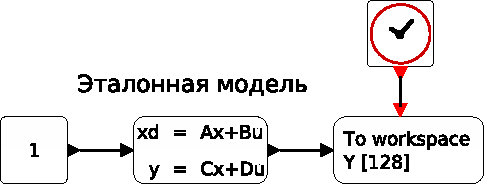
\includegraphics[height = 2.7 cm]{ref_model_scheme.pdf} }
	\end{minipage}
	\hfill
	\begin{minipage}[h]{0.59\linewidth}
		\centering{ 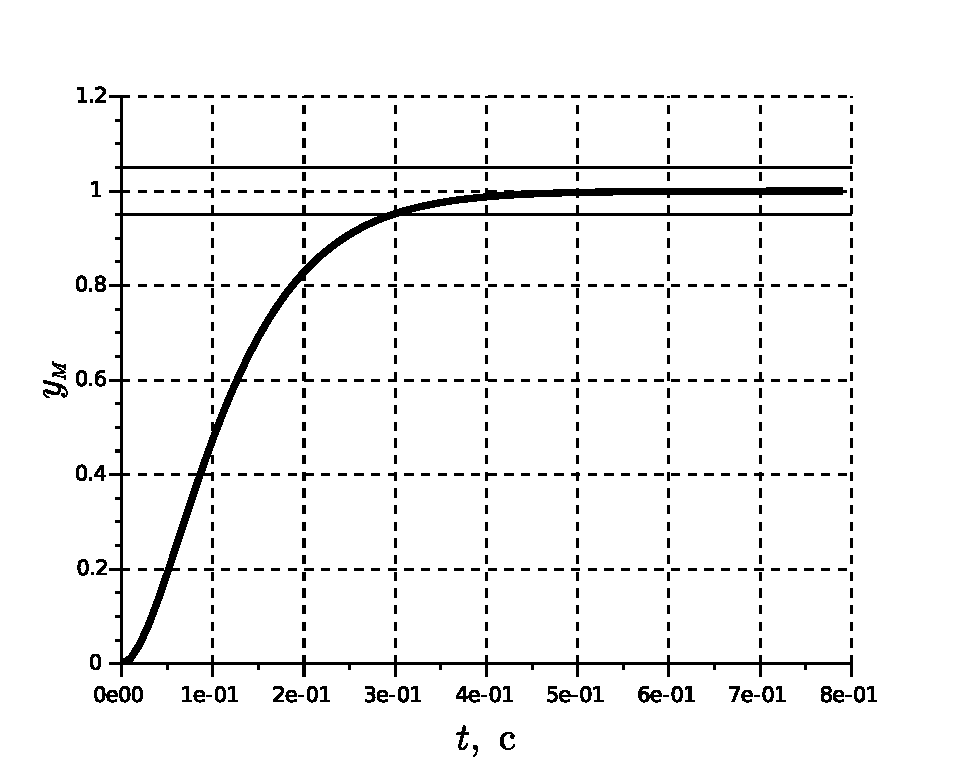
\includegraphics[height = 8.5 cm]{ref_model_trans_func.pdf} }
	\end{minipage}
	\caption{Схема моделирования и график переходной функции эталонной модели.}
	\label{img_ref_model}
\end{figure}

\subsection{Моделирование работы нелинейного закона робастного управления}
Эксперименты с системой робастного управления замкнутой алгоритмом~\ref{eq_tuned_controller},~\ref{AA1} и схема моделирования изображены на рисунках~\ref{img_robust}--\ref{img_r1500d}.
	
\begin{figure}[h!]
	\centering
	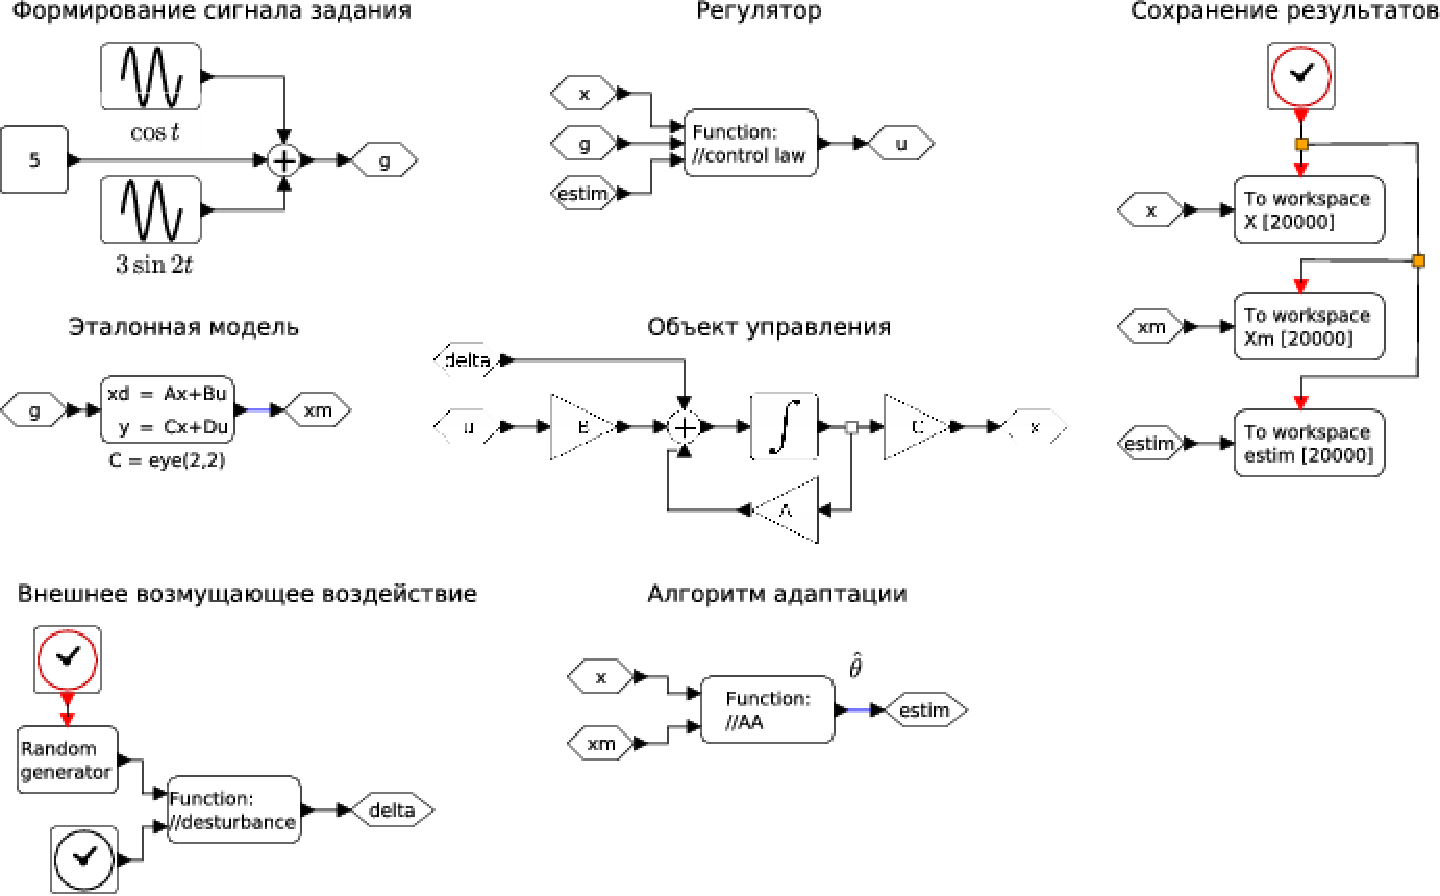
\includegraphics[width=0.79\textwidth]{adapt_desturbance_model_robust.pdf}
	\caption{Схема моделирования процесса работы рассматриваемой системы под управлением АА из п.1}.
	\label{img_robust}
\end{figure}

\begin{figure}[h!]
	\centering
	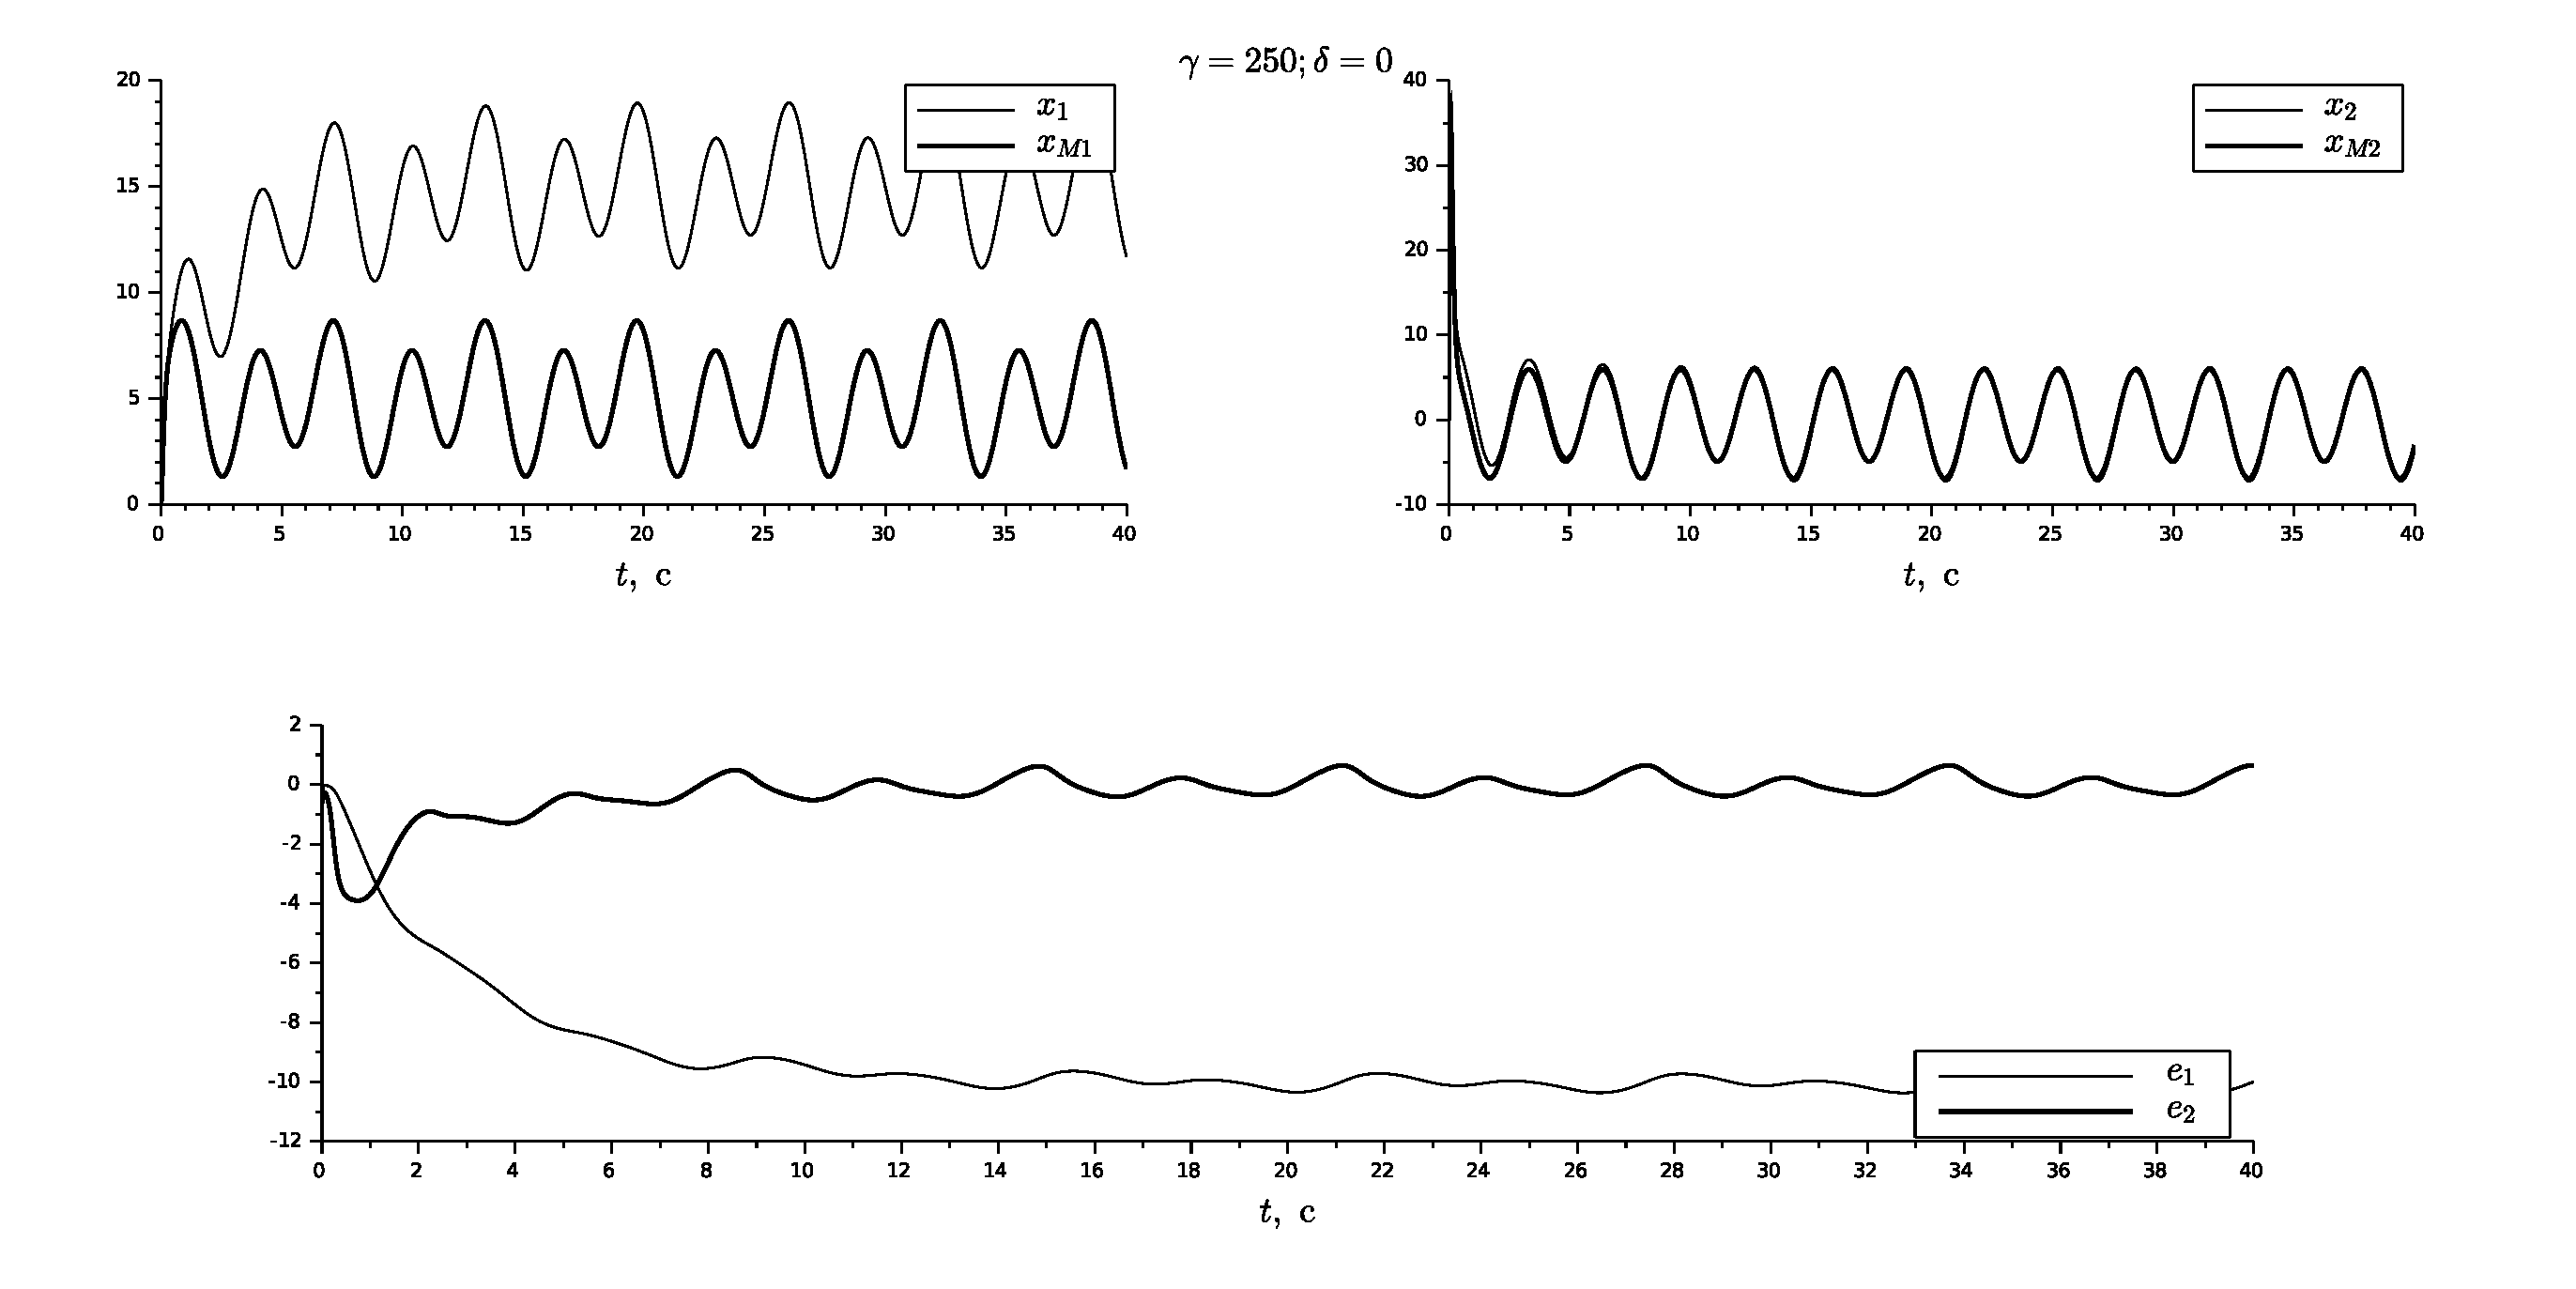
\includegraphics[width=1\textwidth]{robust_250.pdf}
	\caption{Графики переходных процессов без возмущения при $\gamma = 250$}.
	\label{img_r250}
\end{figure}

\begin{figure}[h!]
	\centering
	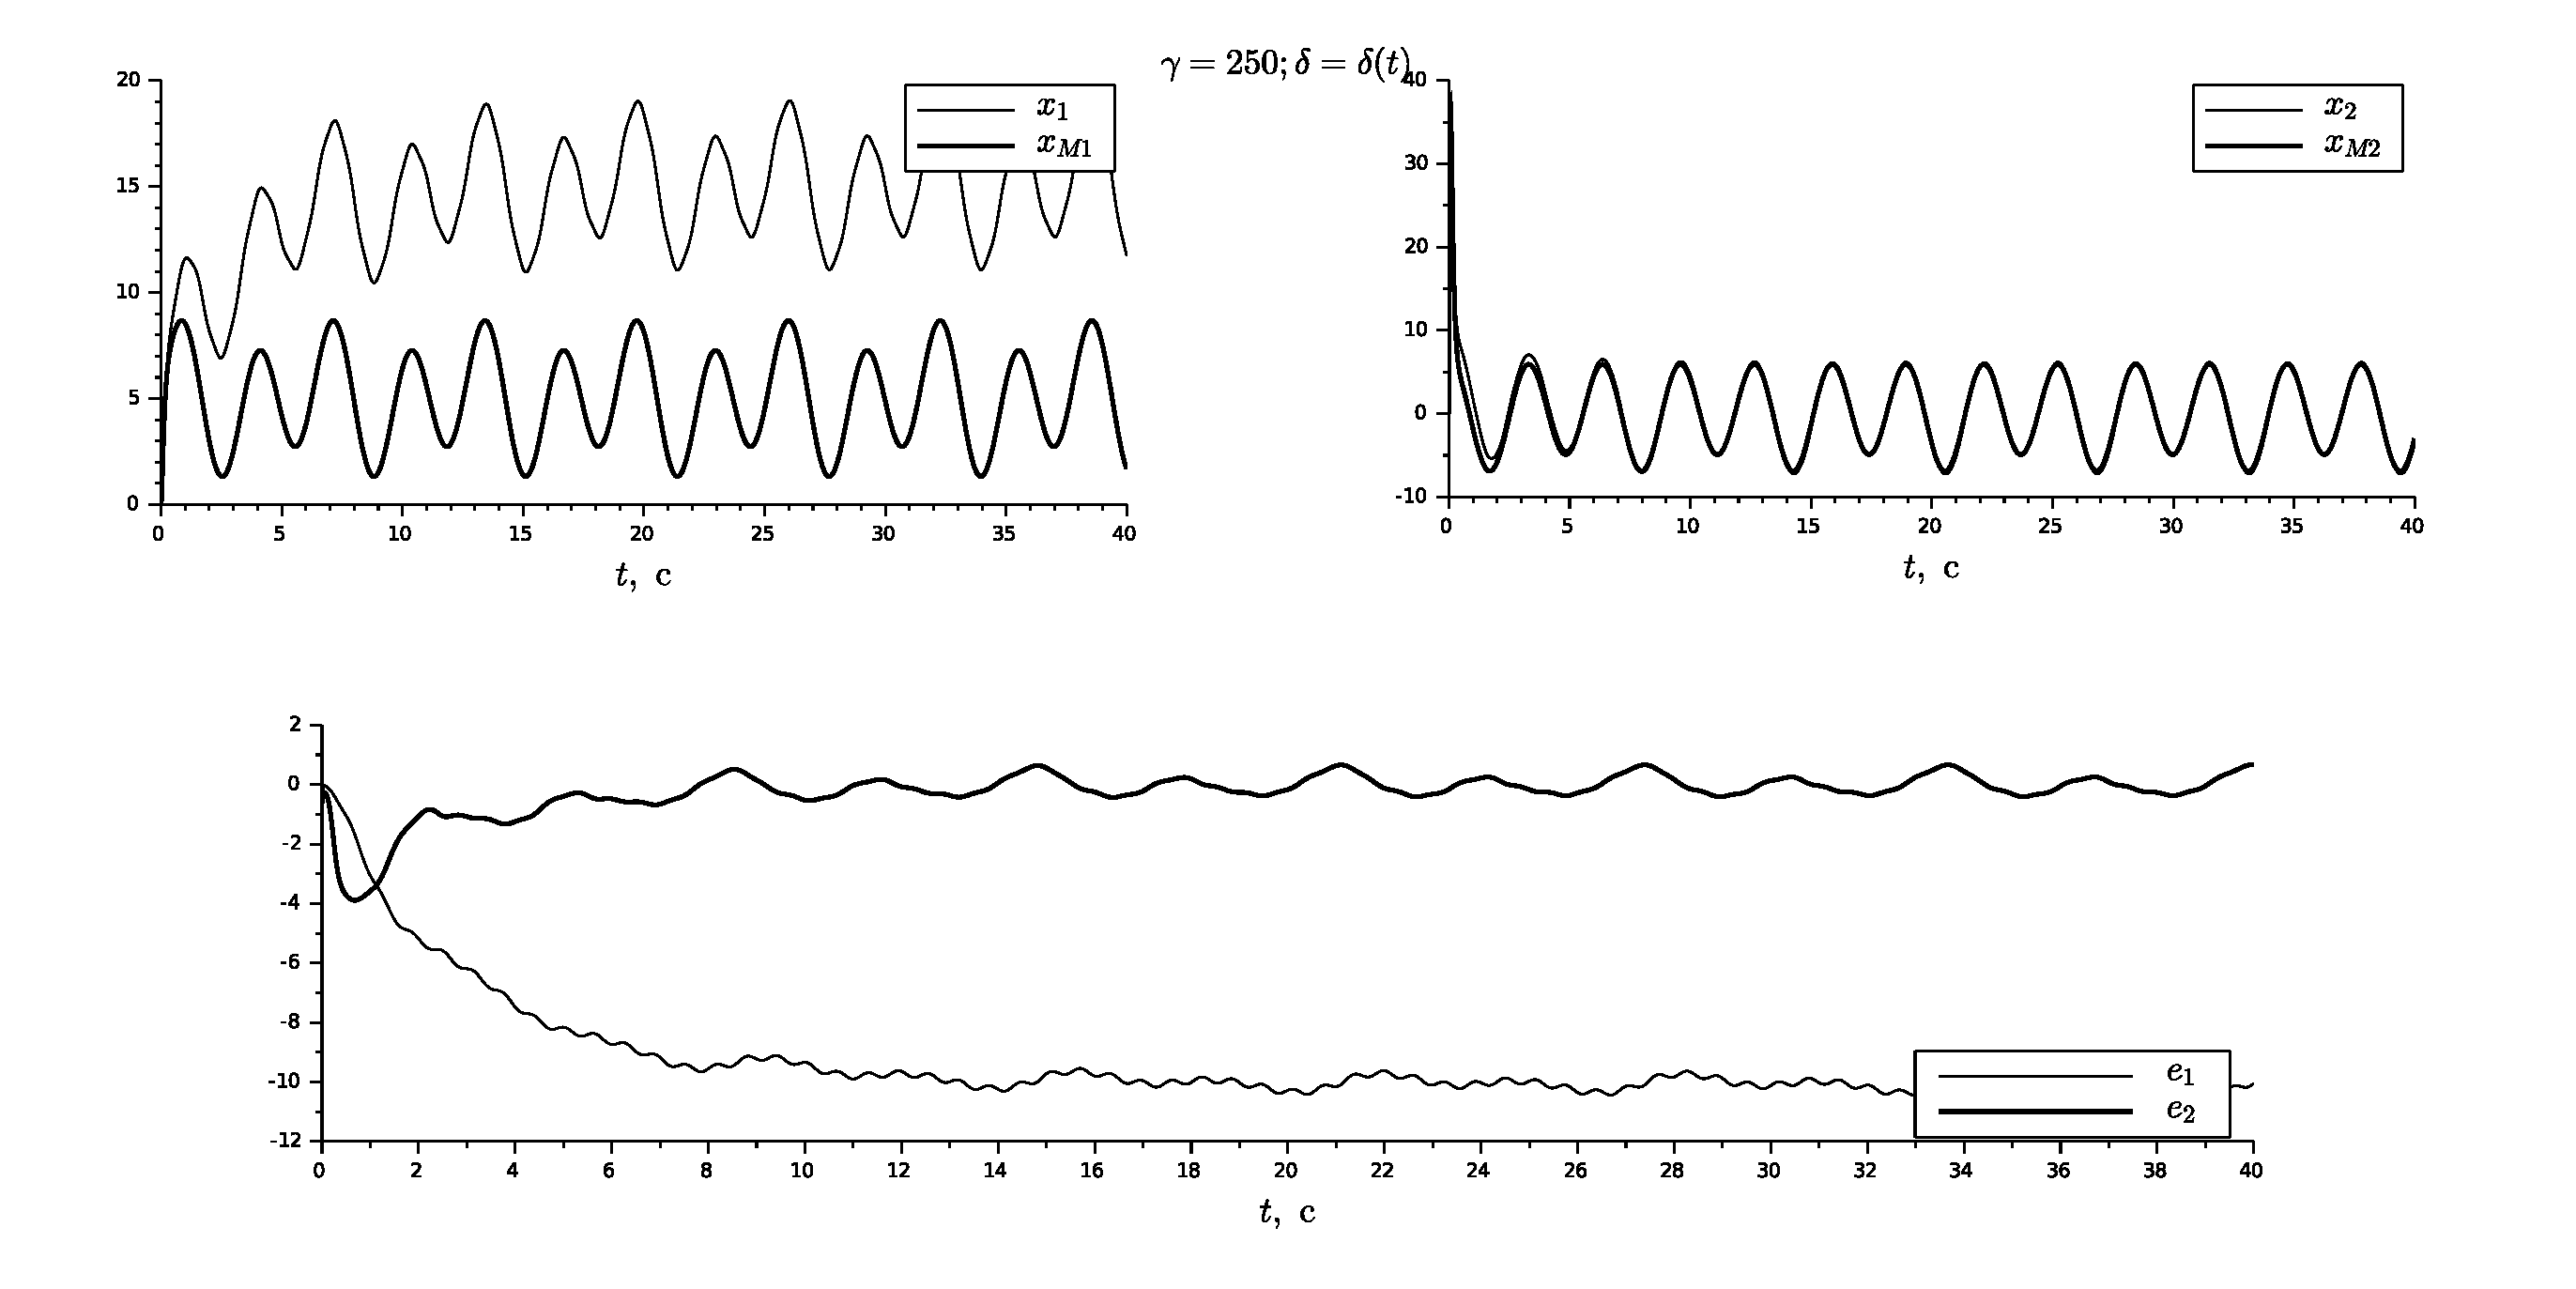
\includegraphics[width=1\textwidth]{robust_250_d.pdf}
	\caption{Графики переходных процессов возмущенной системы при $\gamma = 250$}.
	\label{img_r250d}
\end{figure}

\begin{figure}[h!]
	\centering
	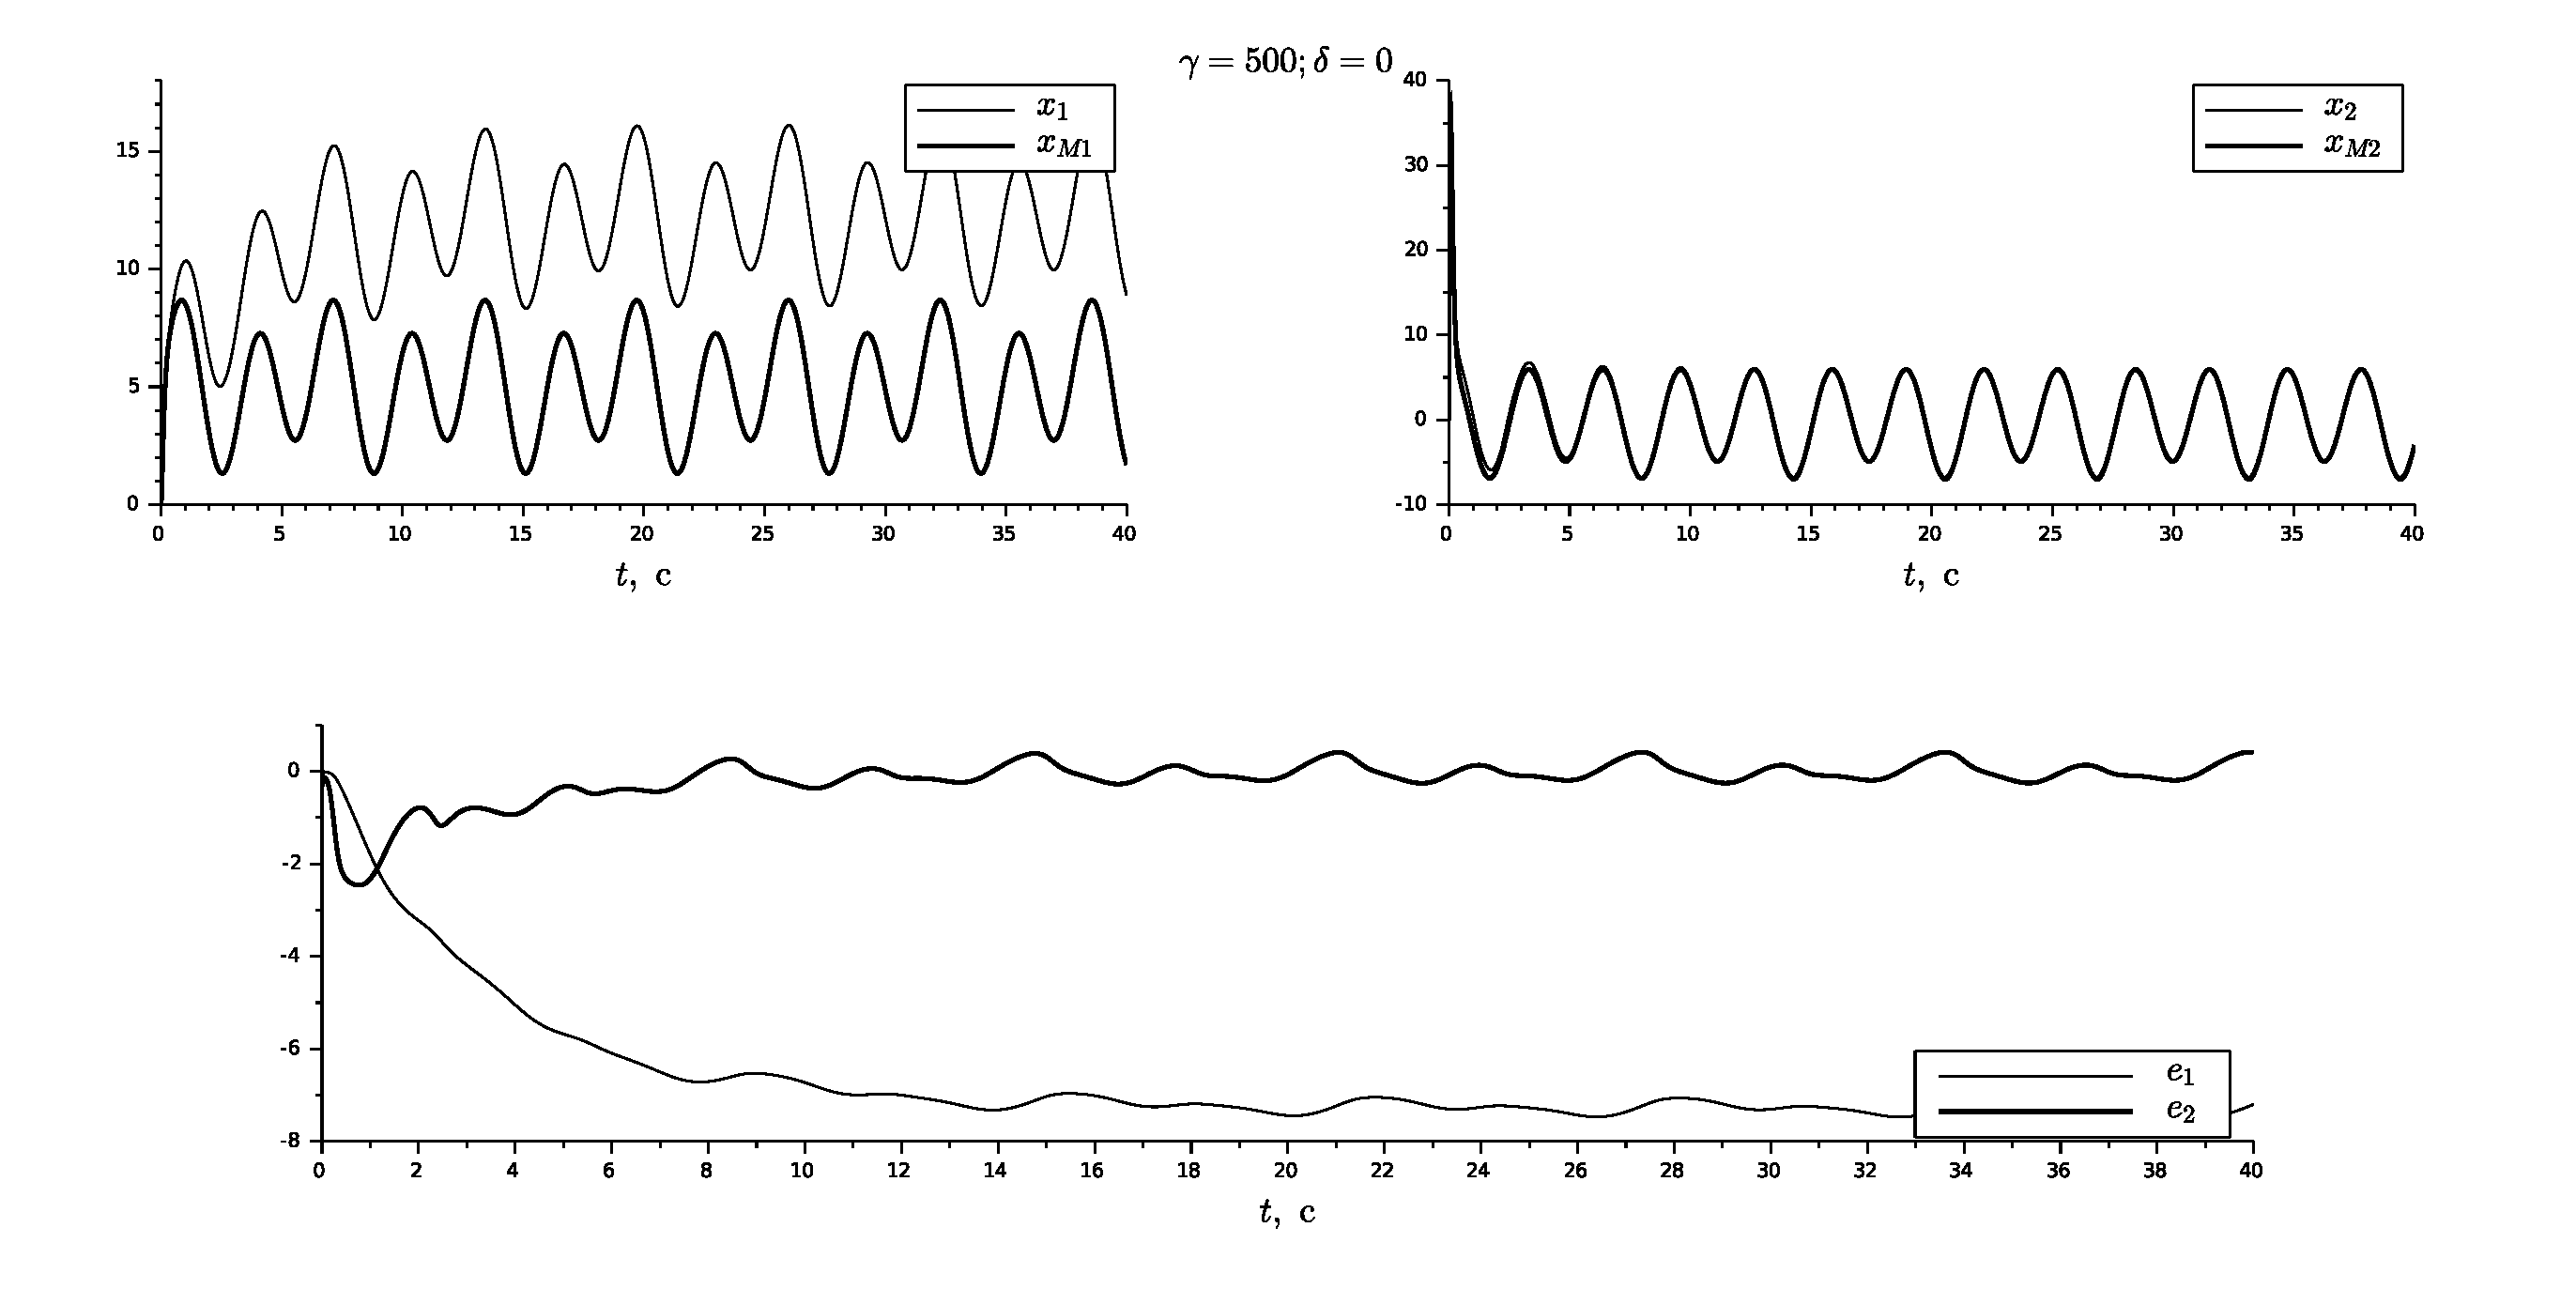
\includegraphics[width=1\textwidth]{robust_500.pdf}
	\caption{Графики переходных процессов без возмущения при $\gamma = 500$}.
	\label{img_r500}
\end{figure}

\begin{figure}[h!]
	\centering
	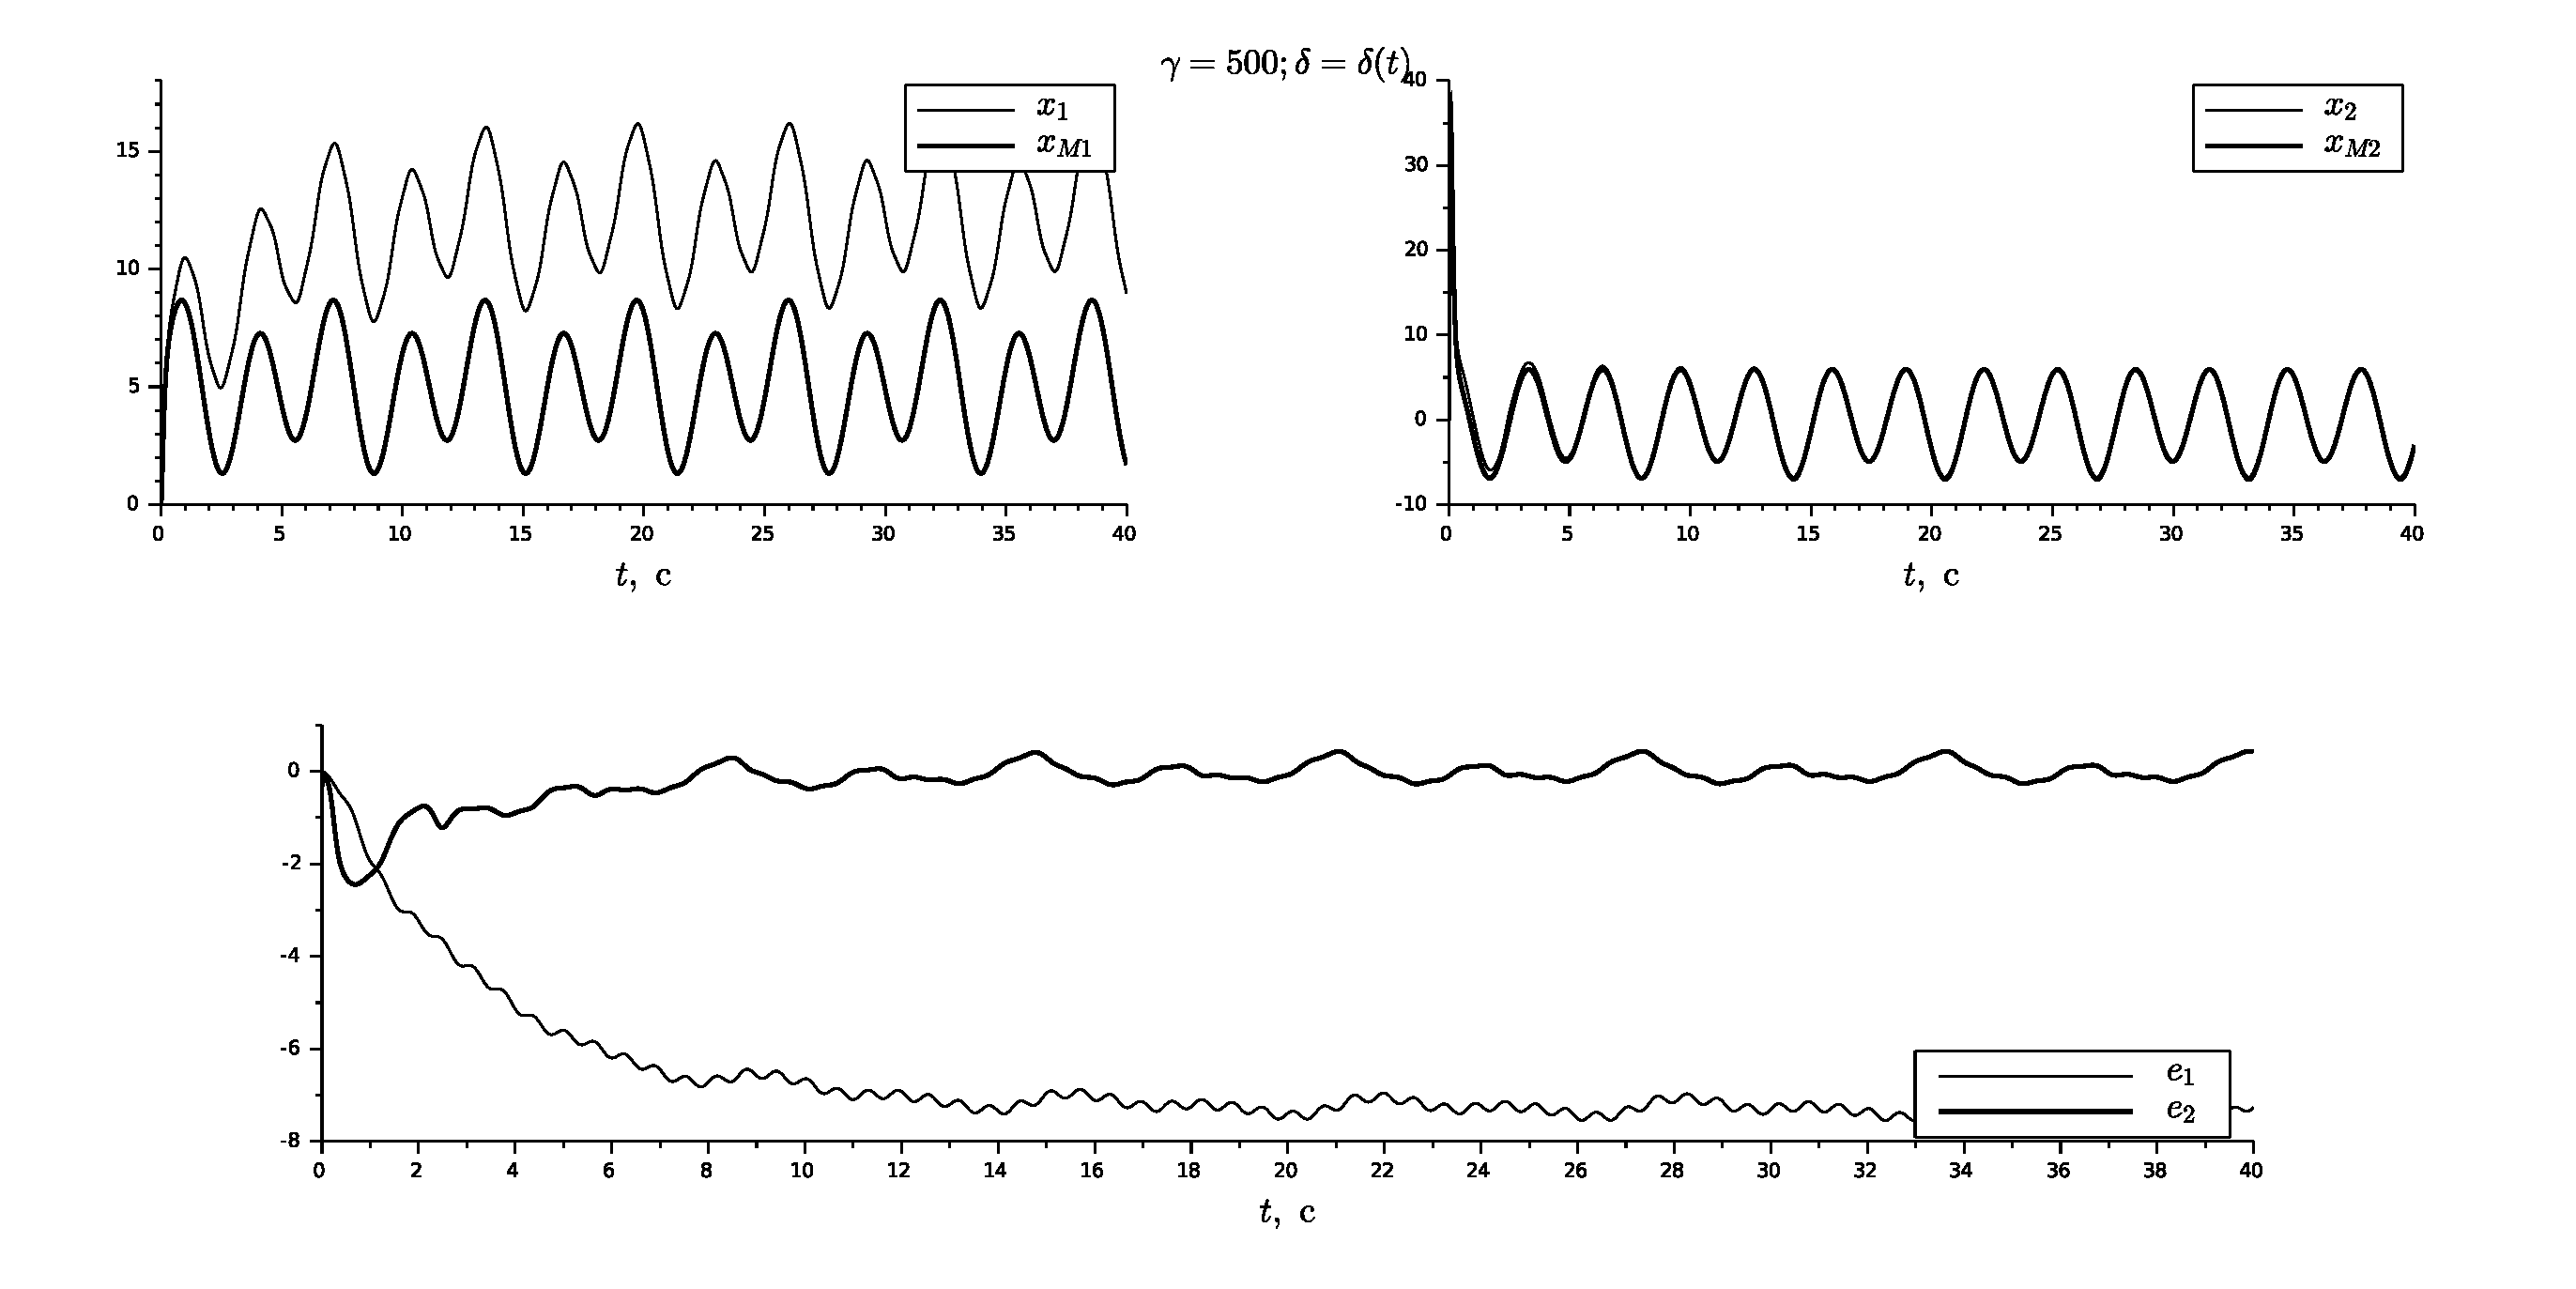
\includegraphics[width=1\textwidth]{robust_500_d.pdf}
	\caption{Графики переходных процессов возмущенной системы при $\gamma = 500$}.
	\label{img_r500d}
\end{figure}

\begin{figure}[h!]
	\centering
	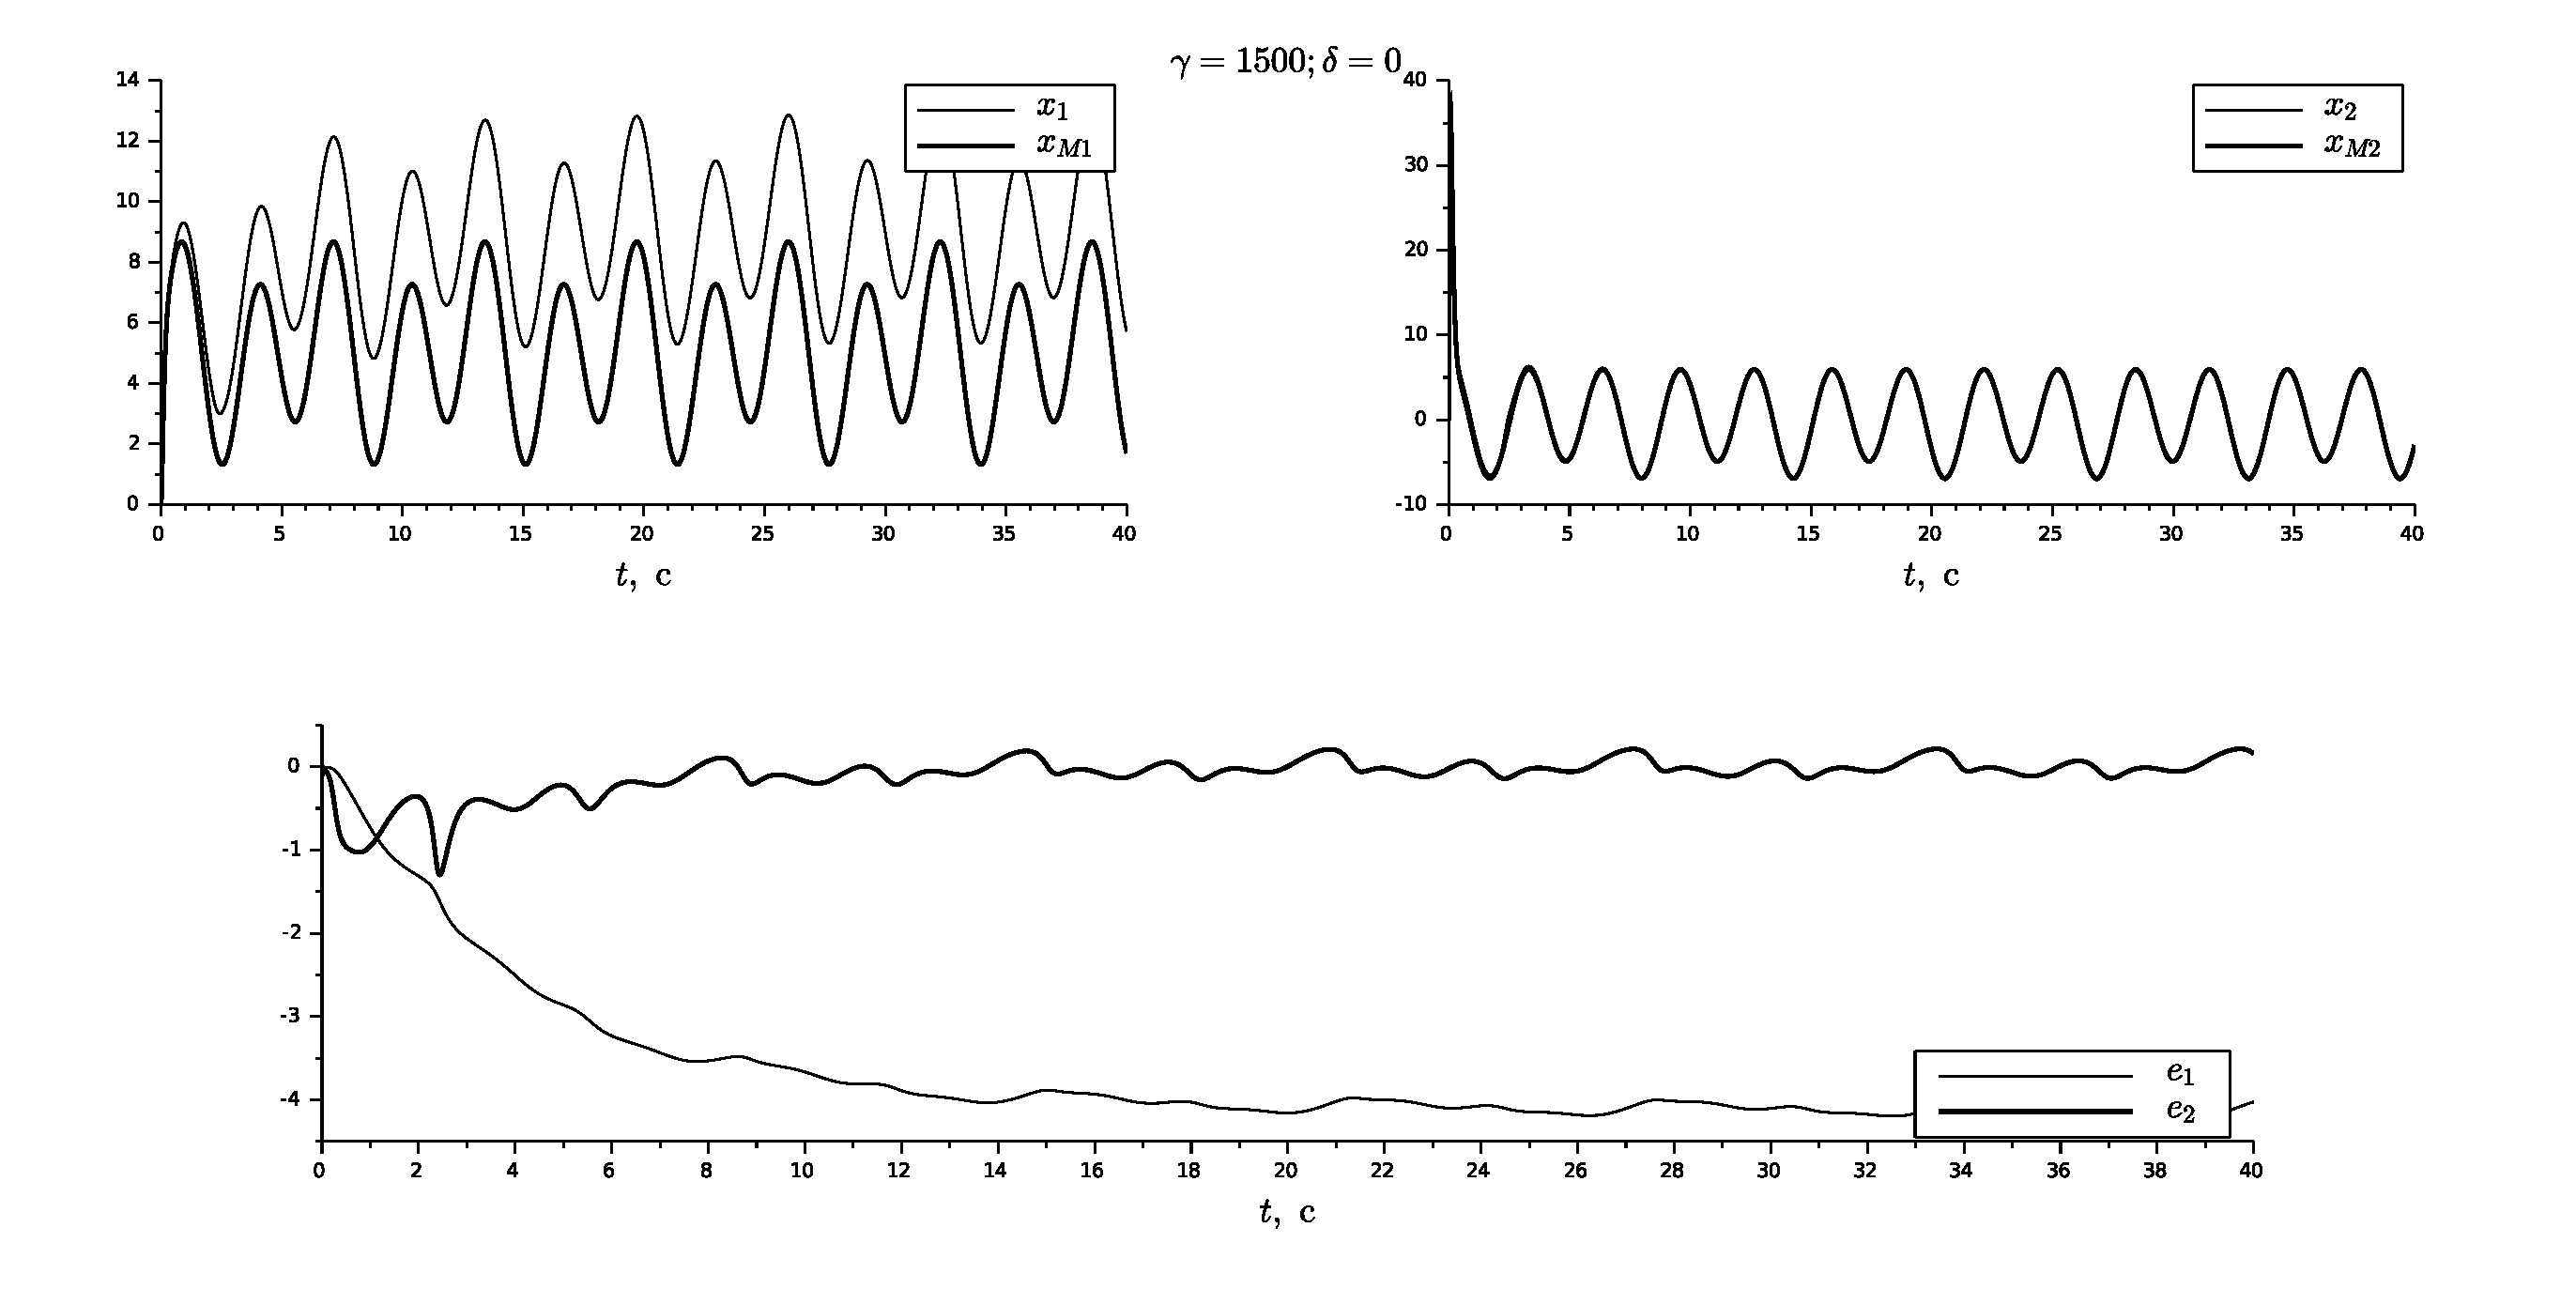
\includegraphics[width=1\textwidth]{robust_1500.pdf}
	\caption{Графики переходных процессов без возмущения при $\gamma = 1500$}.
	\label{img_r1500}
\end{figure}

\begin{figure}[h!]
	\centering
	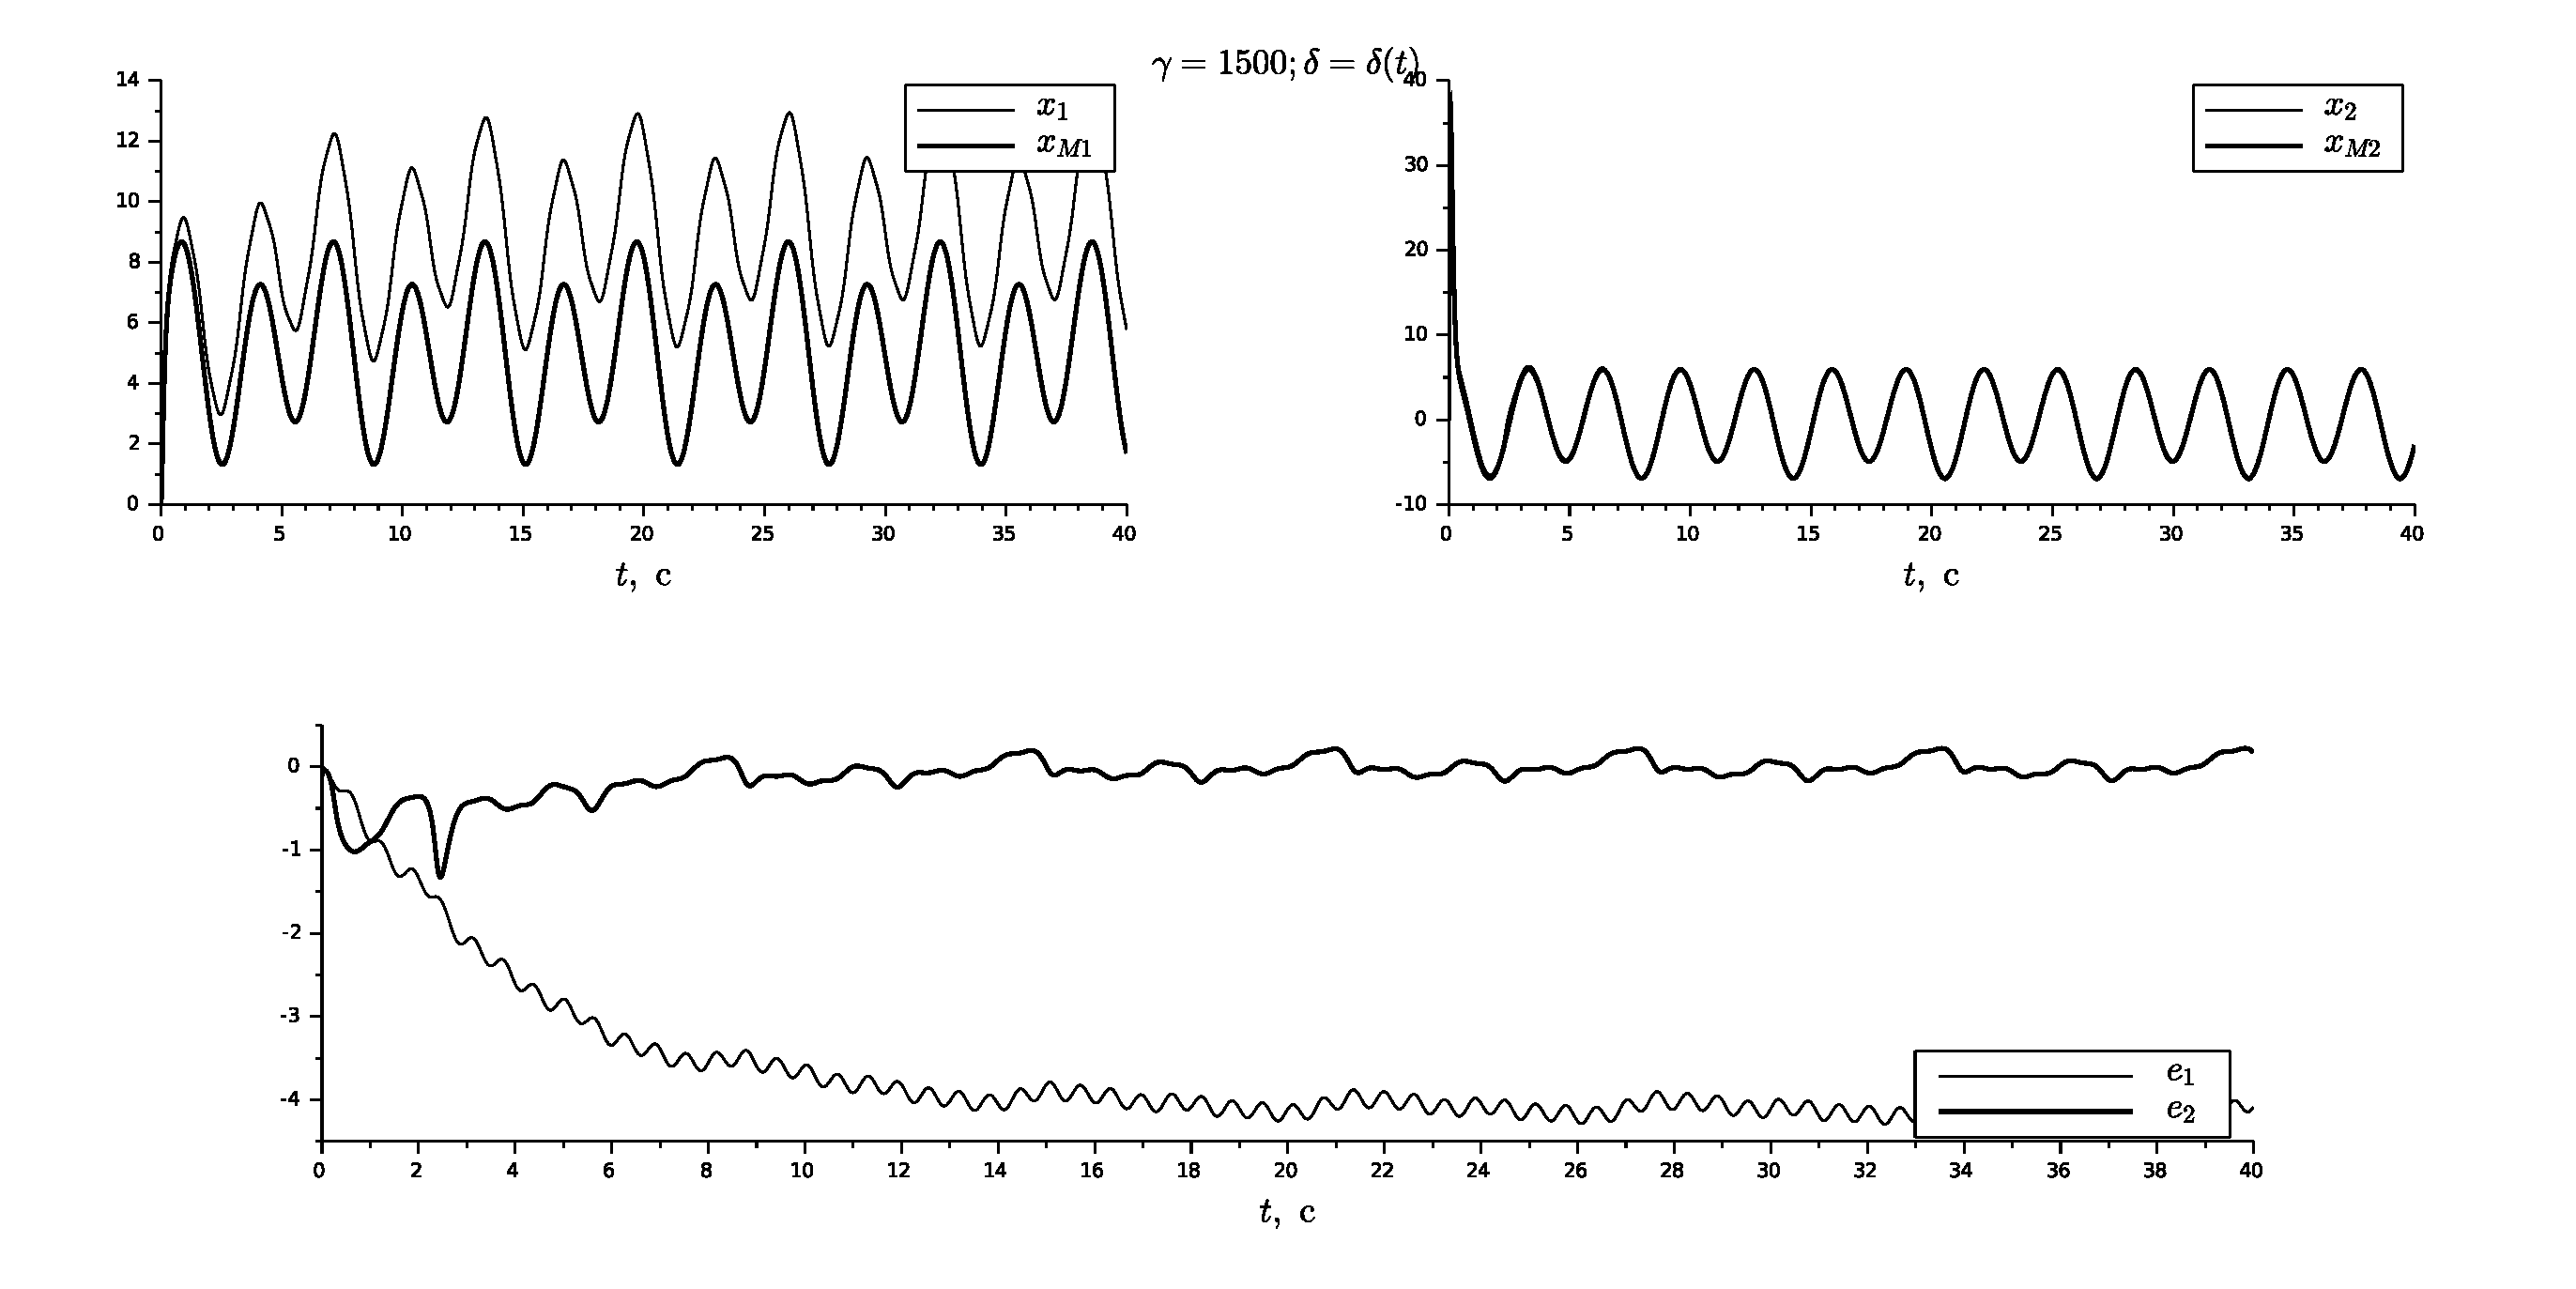
\includegraphics[width=1\textwidth]{robust_1500_d.pdf}
	\caption{Графики переходных процессов возмущенной системы при $\gamma = 1500$}.
	\label{img_r1500d}
\end{figure}


\clearpage
\newpage
\subsection{Моделирование работы адаптивного и робастного управления}
Эксперименты с системой адаптивного и робастного управления замкнутой алгоритмом~\ref{eq_tuned_controller},~\ref{AA2} и схема моделирования изображены на рисунках~\ref{img_adapt_and_robust_model}--\ref{img_s01ar1500_d2}.

\begin{figure}[h!]
	\centering
	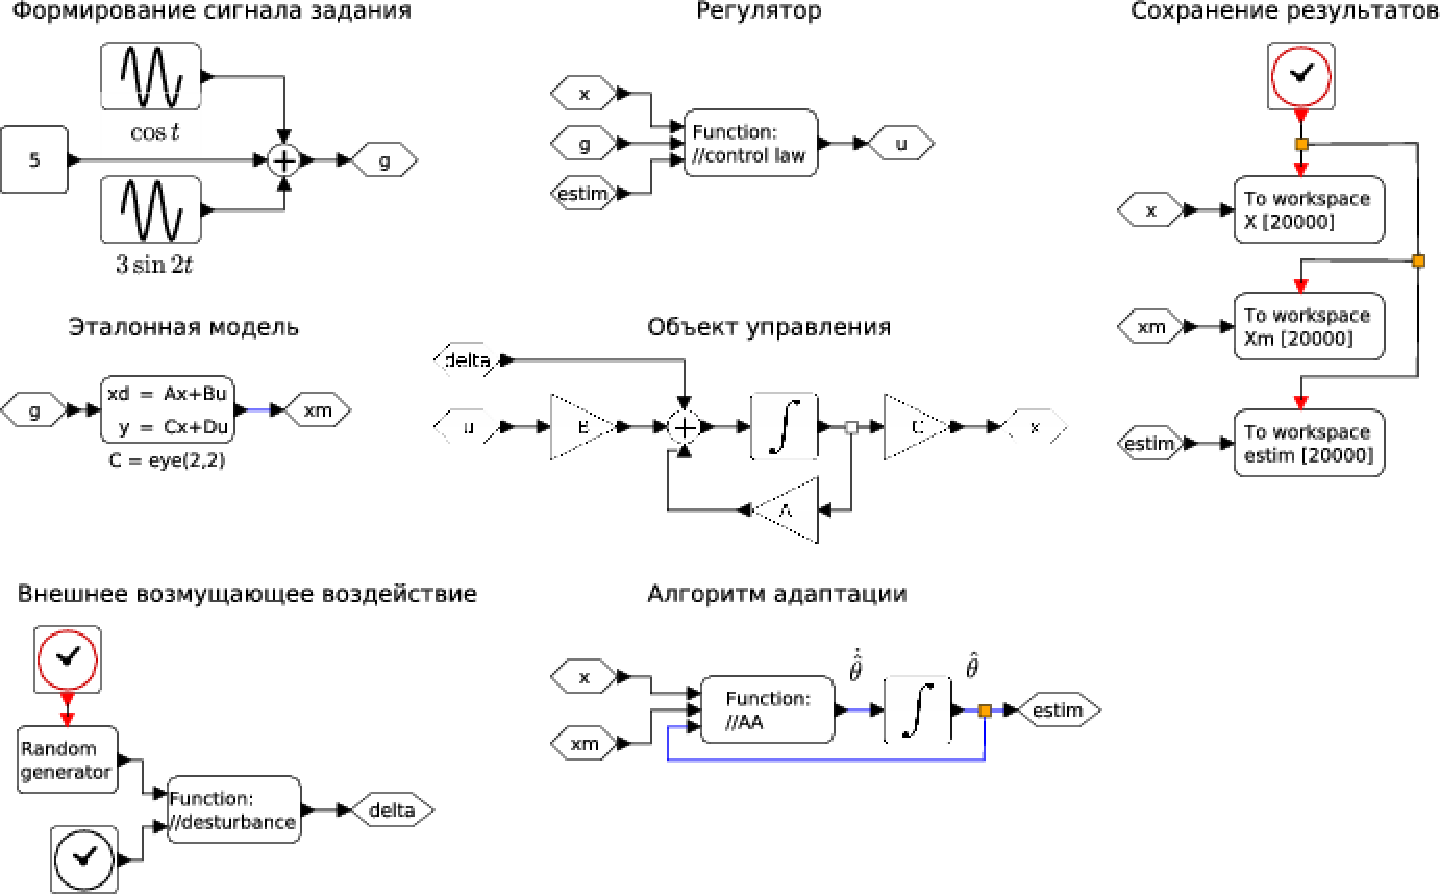
\includegraphics[width=1\textwidth]{adapt_desturbance_model_robust_and_adapt.pdf}
	\caption{Схема моделирования адаптивной и робастной системы}
	\label{img_adapt_and_robust_model}
\end{figure}

На рисунках~\ref{img_ar250}--\ref{img_ar1500_d2} приведены графики моделирования для $\sigma = 0.2$. После них, на рисунках~\ref{img_s01ar1500}--\ref{img_s01ar1500_d2} приведены графики моделирования для $\sigma = 0.01$.

\begin{figure}[h!]
	\centering
	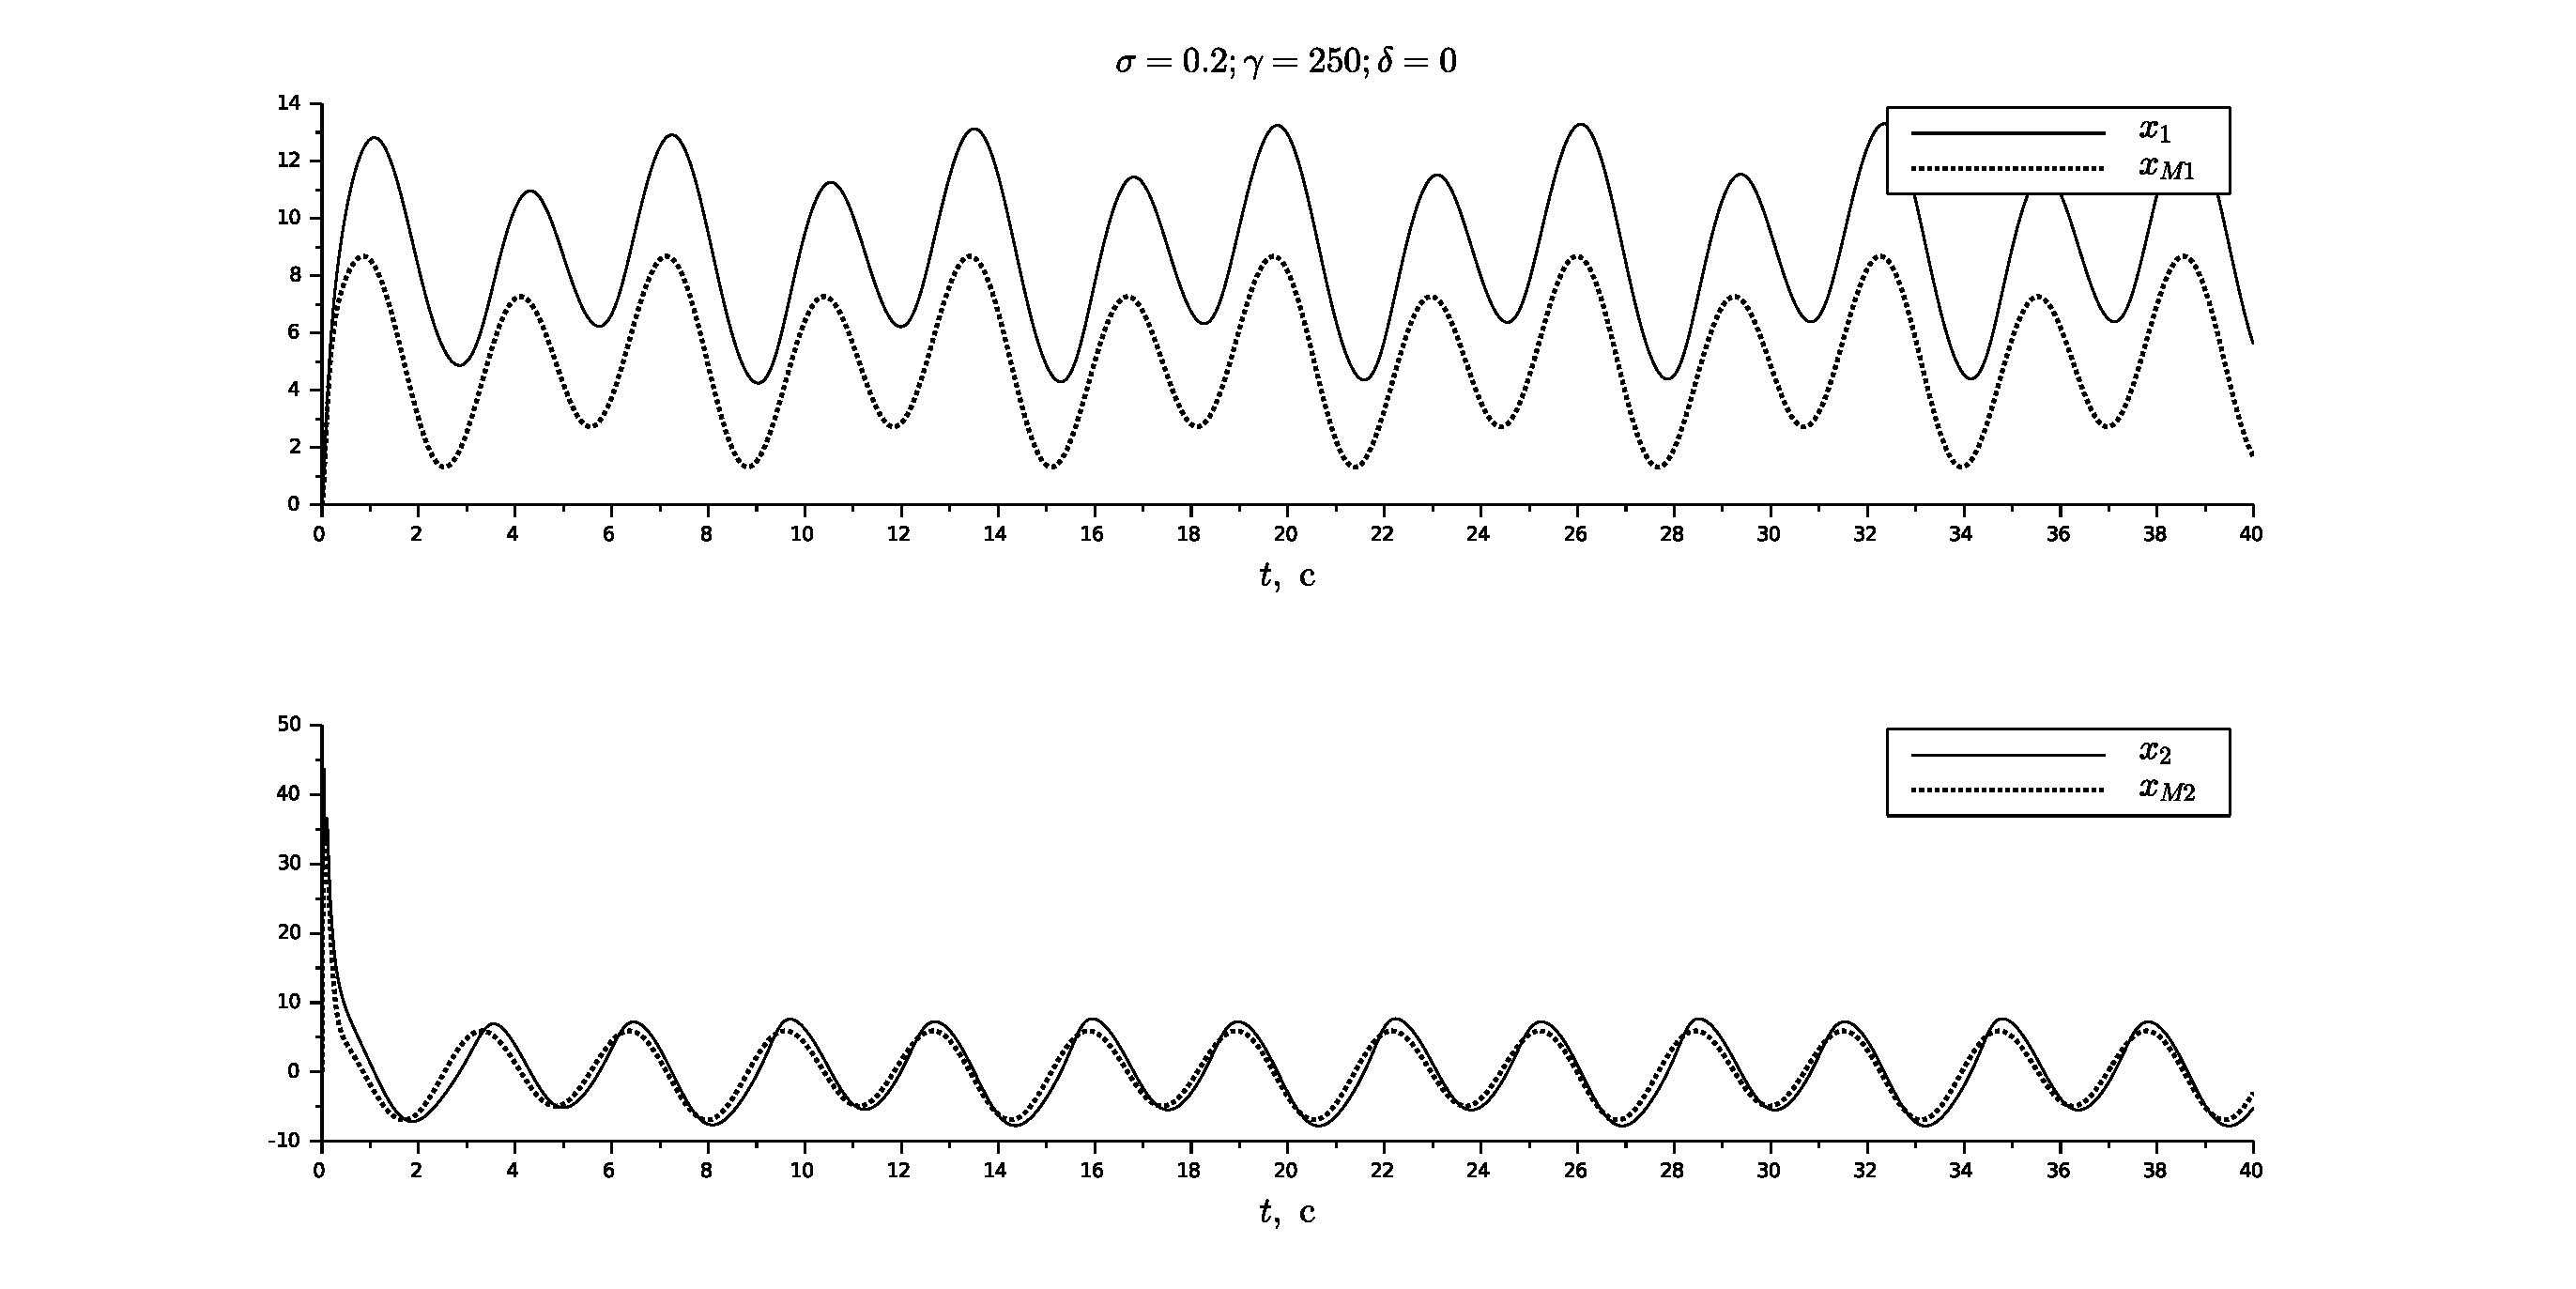
\includegraphics[width=1\textwidth]{arobust_250_1.pdf}
	\caption{Графики переходных процессов невозмущенной системы при $\sigma = 0.2, \gamma = 250$}
	\label{img_ar250}
\end{figure}

\begin{figure}[h!]
	\centering
	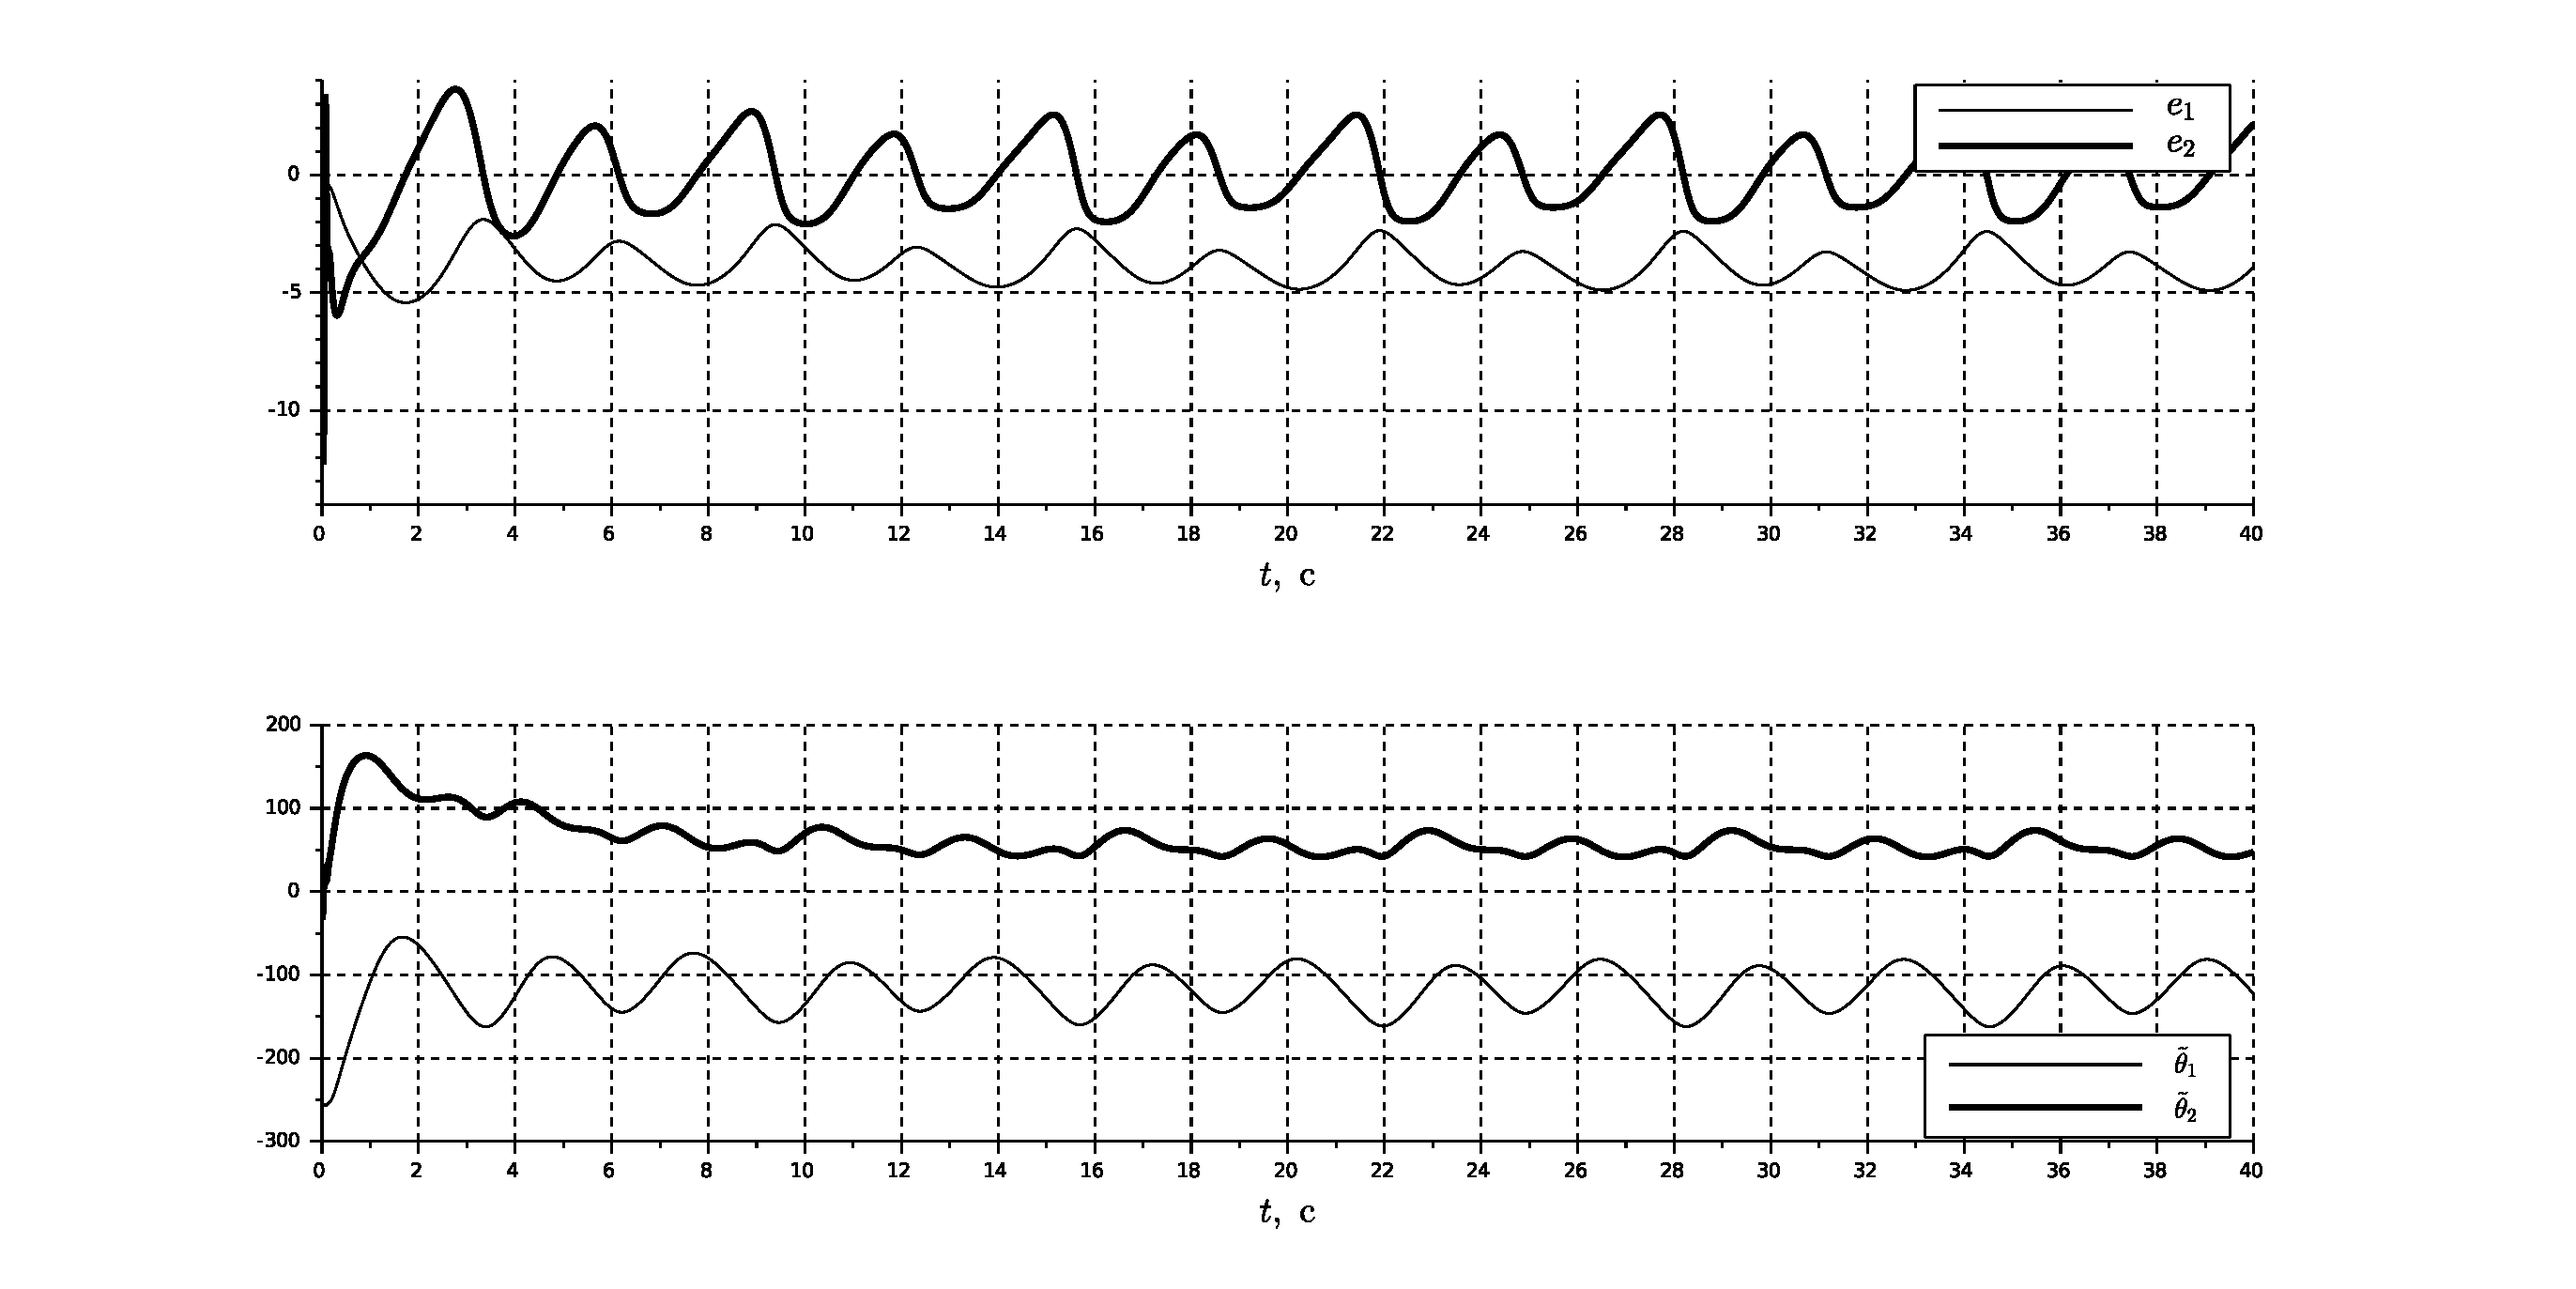
\includegraphics[width=1\textwidth]{arobust_250_2.pdf}
	\caption{Графики ошибок вектора состояния и параметров невозмущенной системы при $\sigma = 0.2, \gamma = 250$}
	\label{img_ar250_2}
\end{figure}

\begin{figure}[h!]
	\centering
	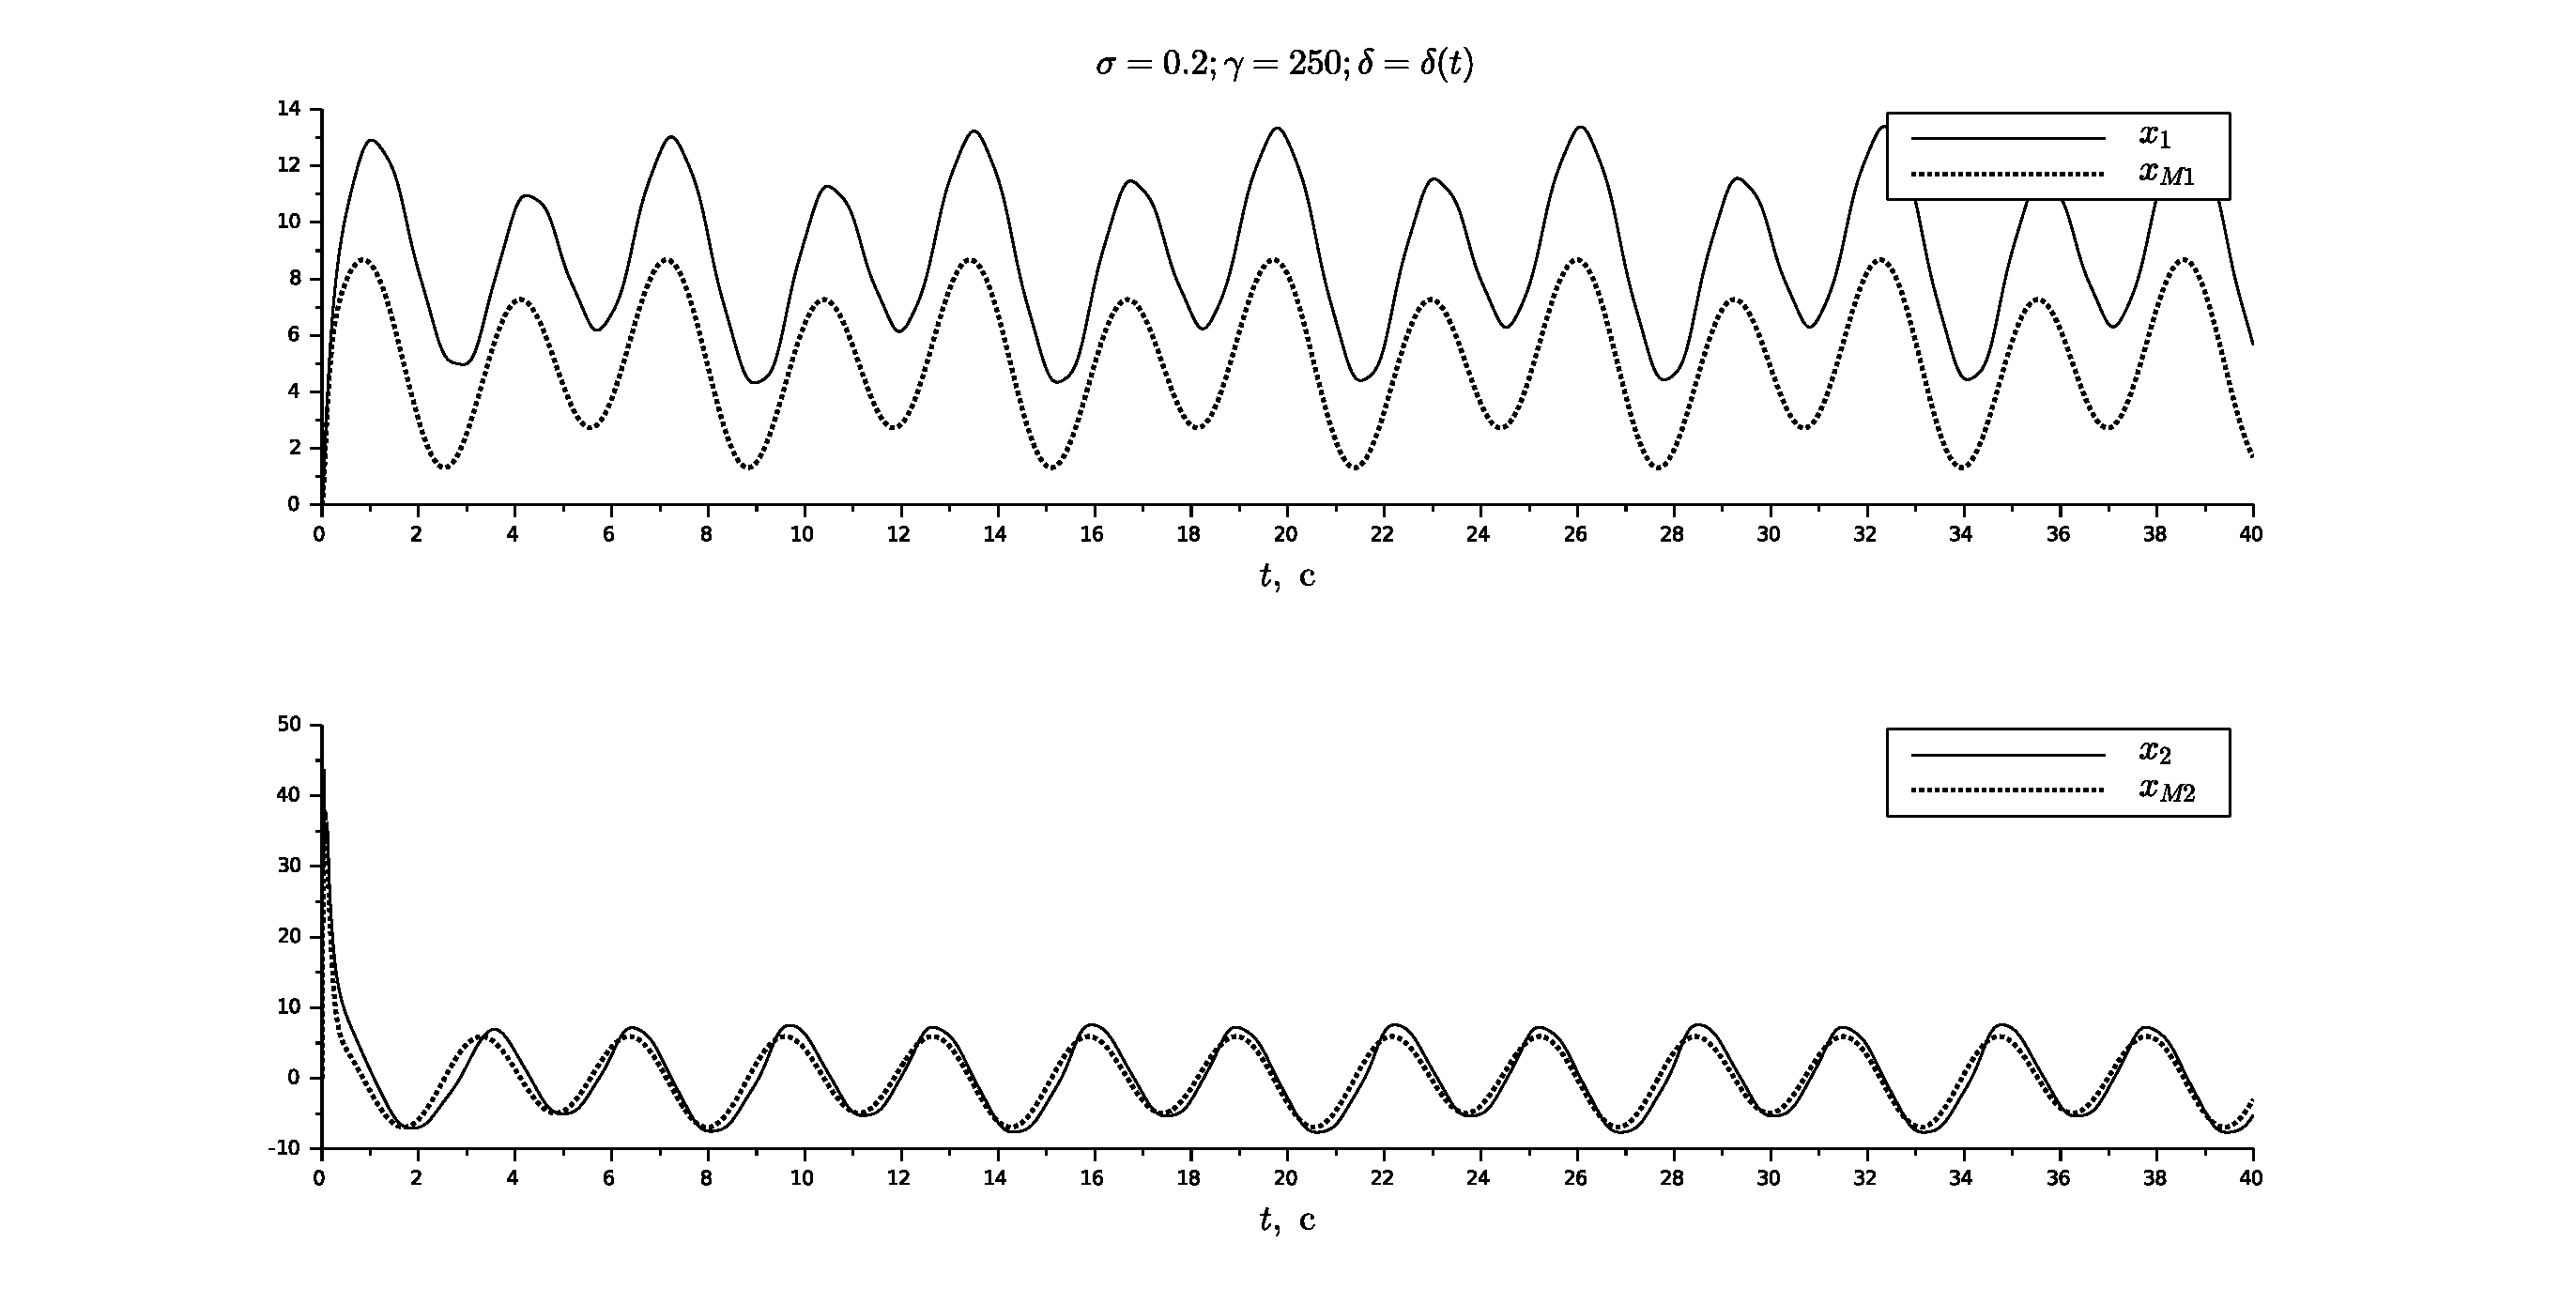
\includegraphics[width=1\textwidth]{arobust_250_d_1.pdf}
	\caption{Графики переходных процессов возмущенной системы при $\sigma = 0.2, \gamma = 250$}
	\label{img_ar250d}
\end{figure}

\begin{figure}[h!]
	\centering
	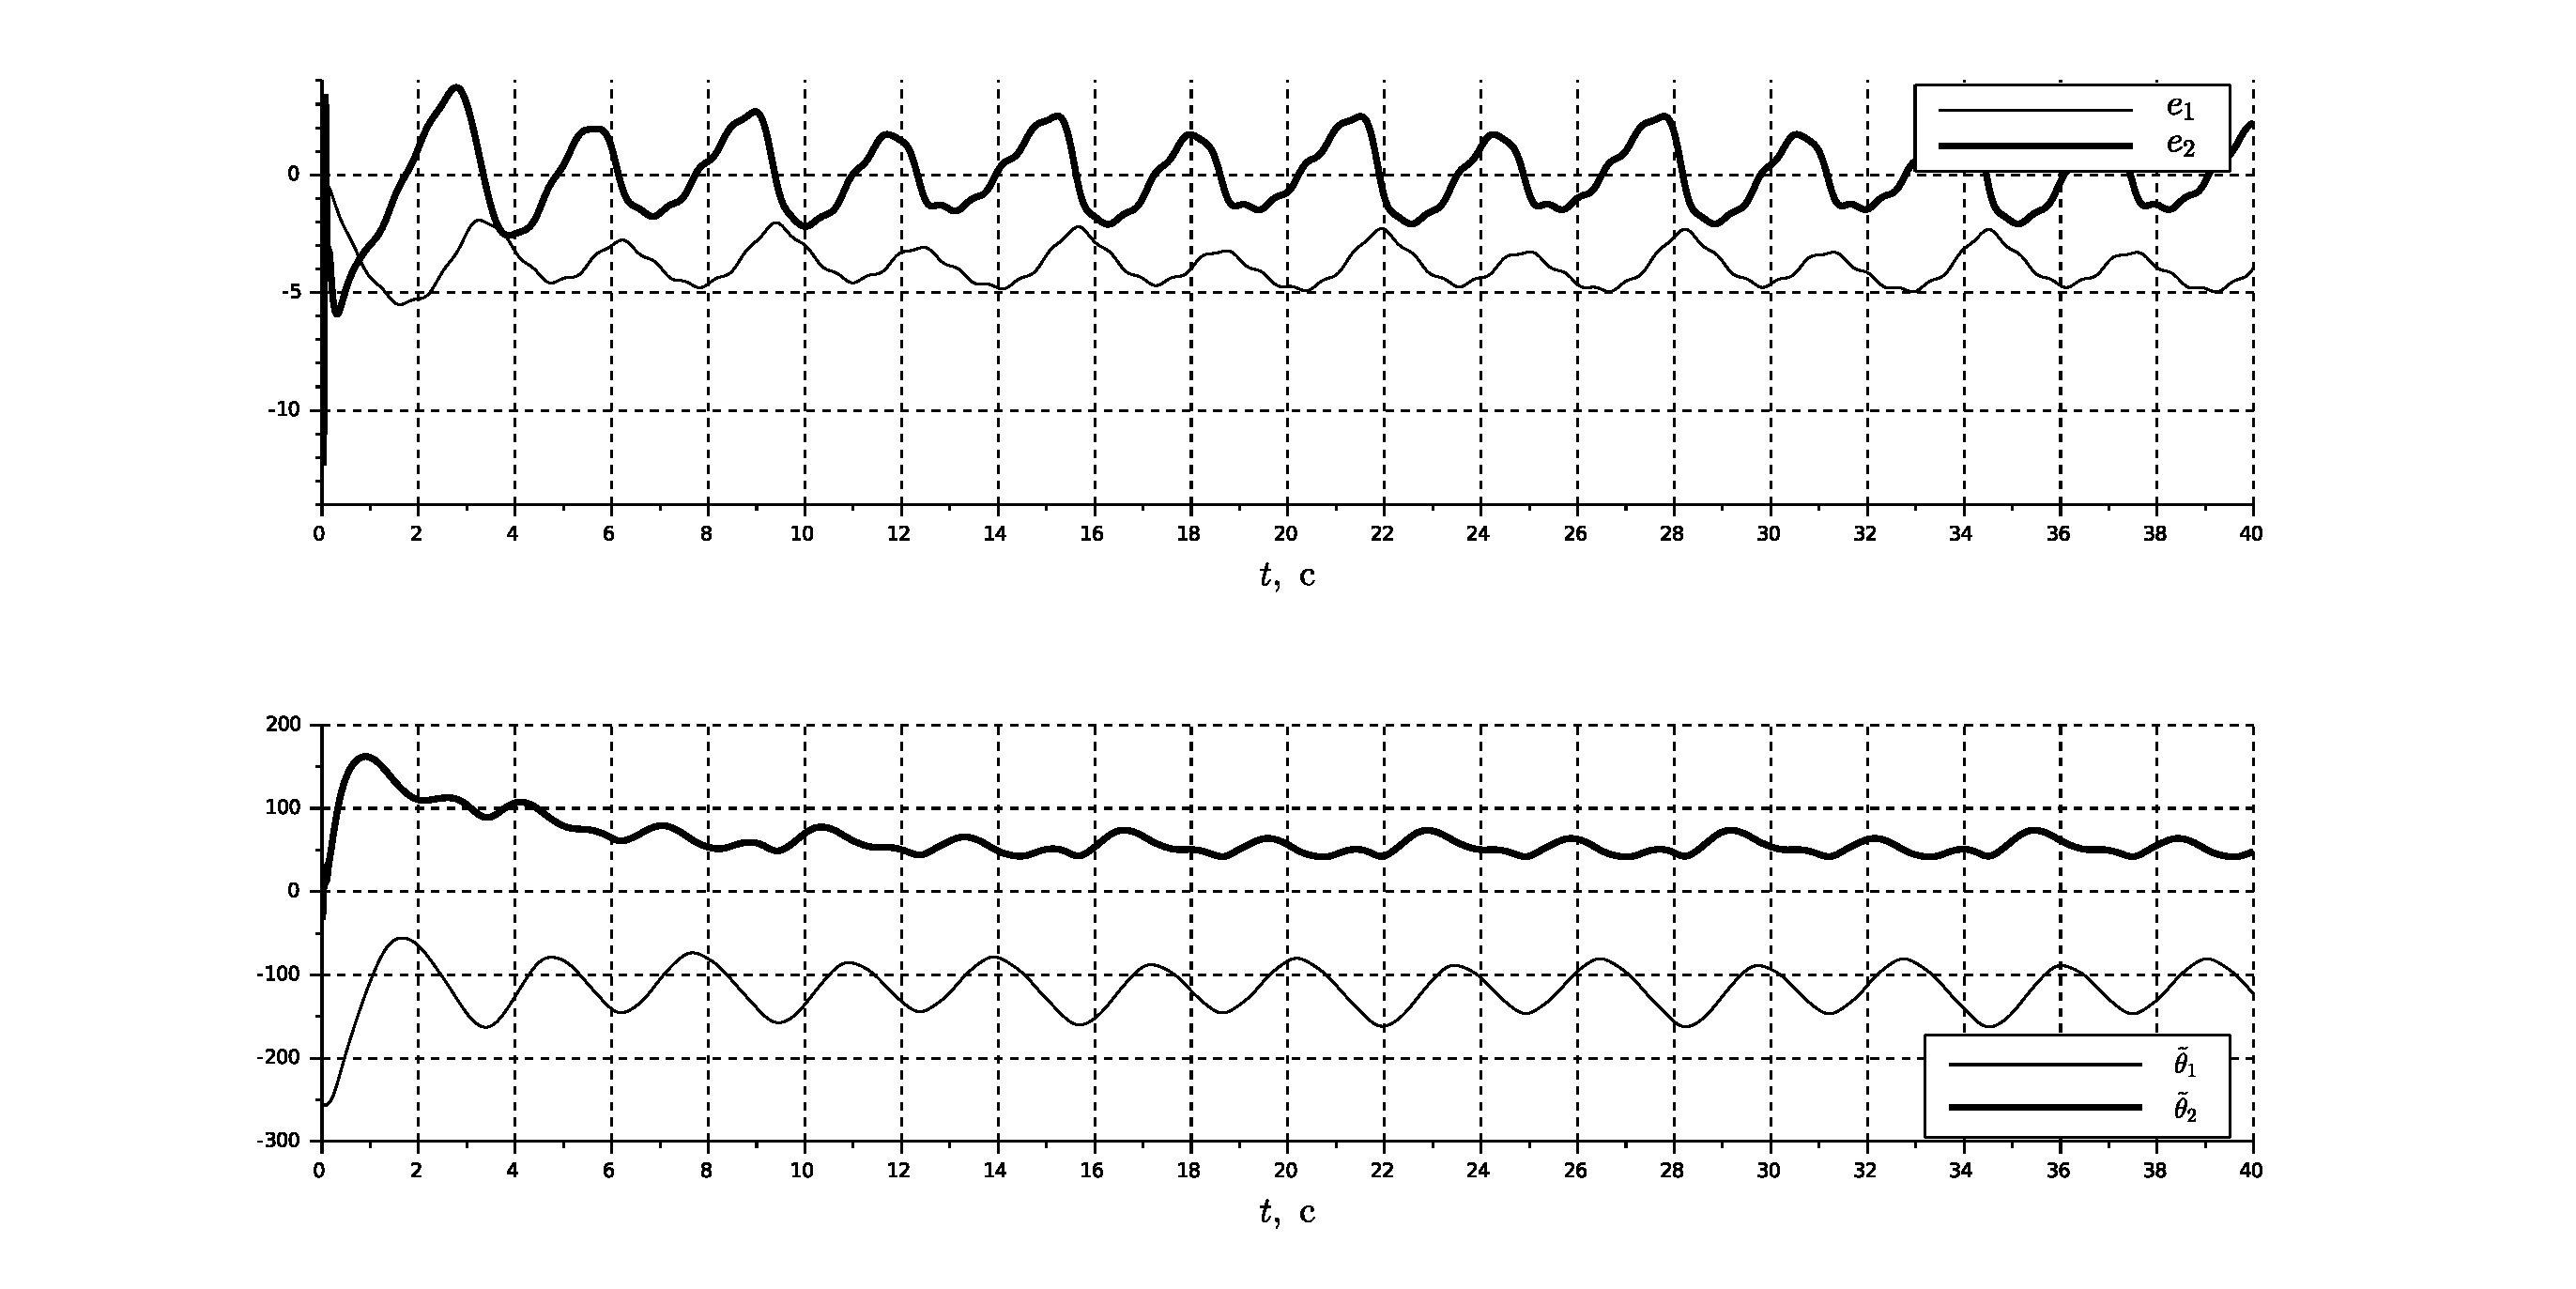
\includegraphics[width=1\textwidth]{arobust_250_d_2.pdf}
	\caption{Графики ошибок вектора состояния и параметров возмущенной системы при $\sigma = 0.2, \gamma = 250$}
	\label{img_ar250_d2}
\end{figure}

\begin{figure}[h!]
	\centering
	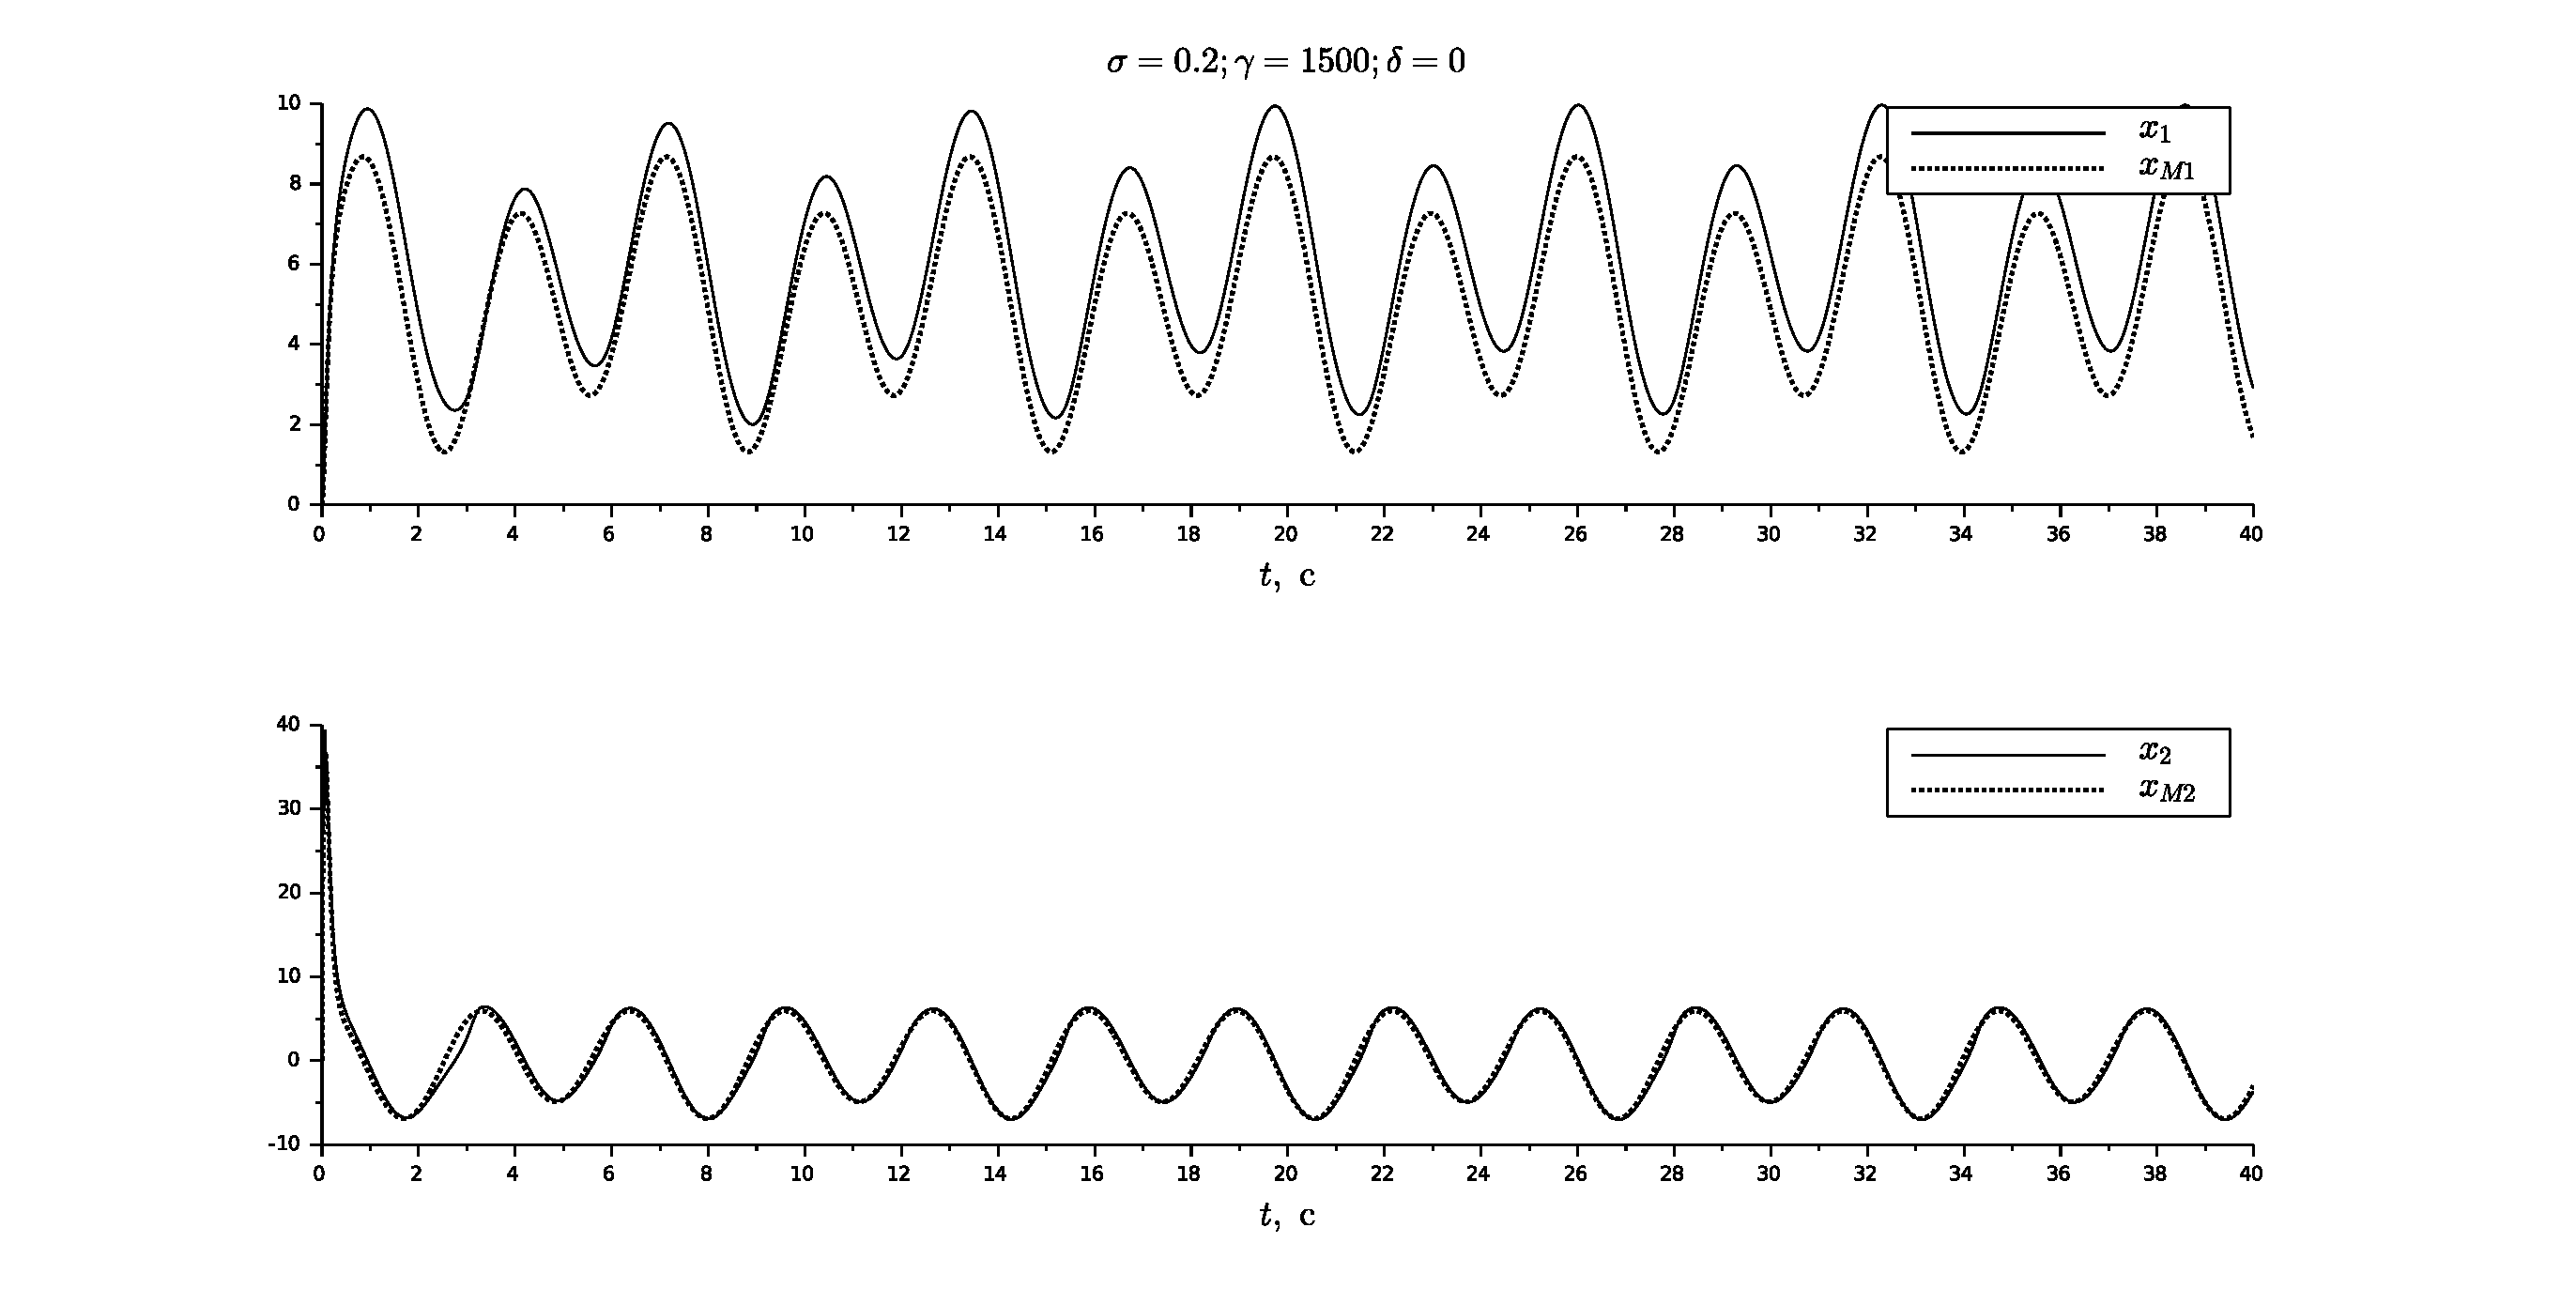
\includegraphics[width=1\textwidth]{arobust_1500_1.pdf}
	\caption{Графики переходных процессов невозмущенной системы при $\sigma = 0.2, \gamma = 1500$}
	\label{img_ar1500}
\end{figure}

\begin{figure}[h!]
	\centering
	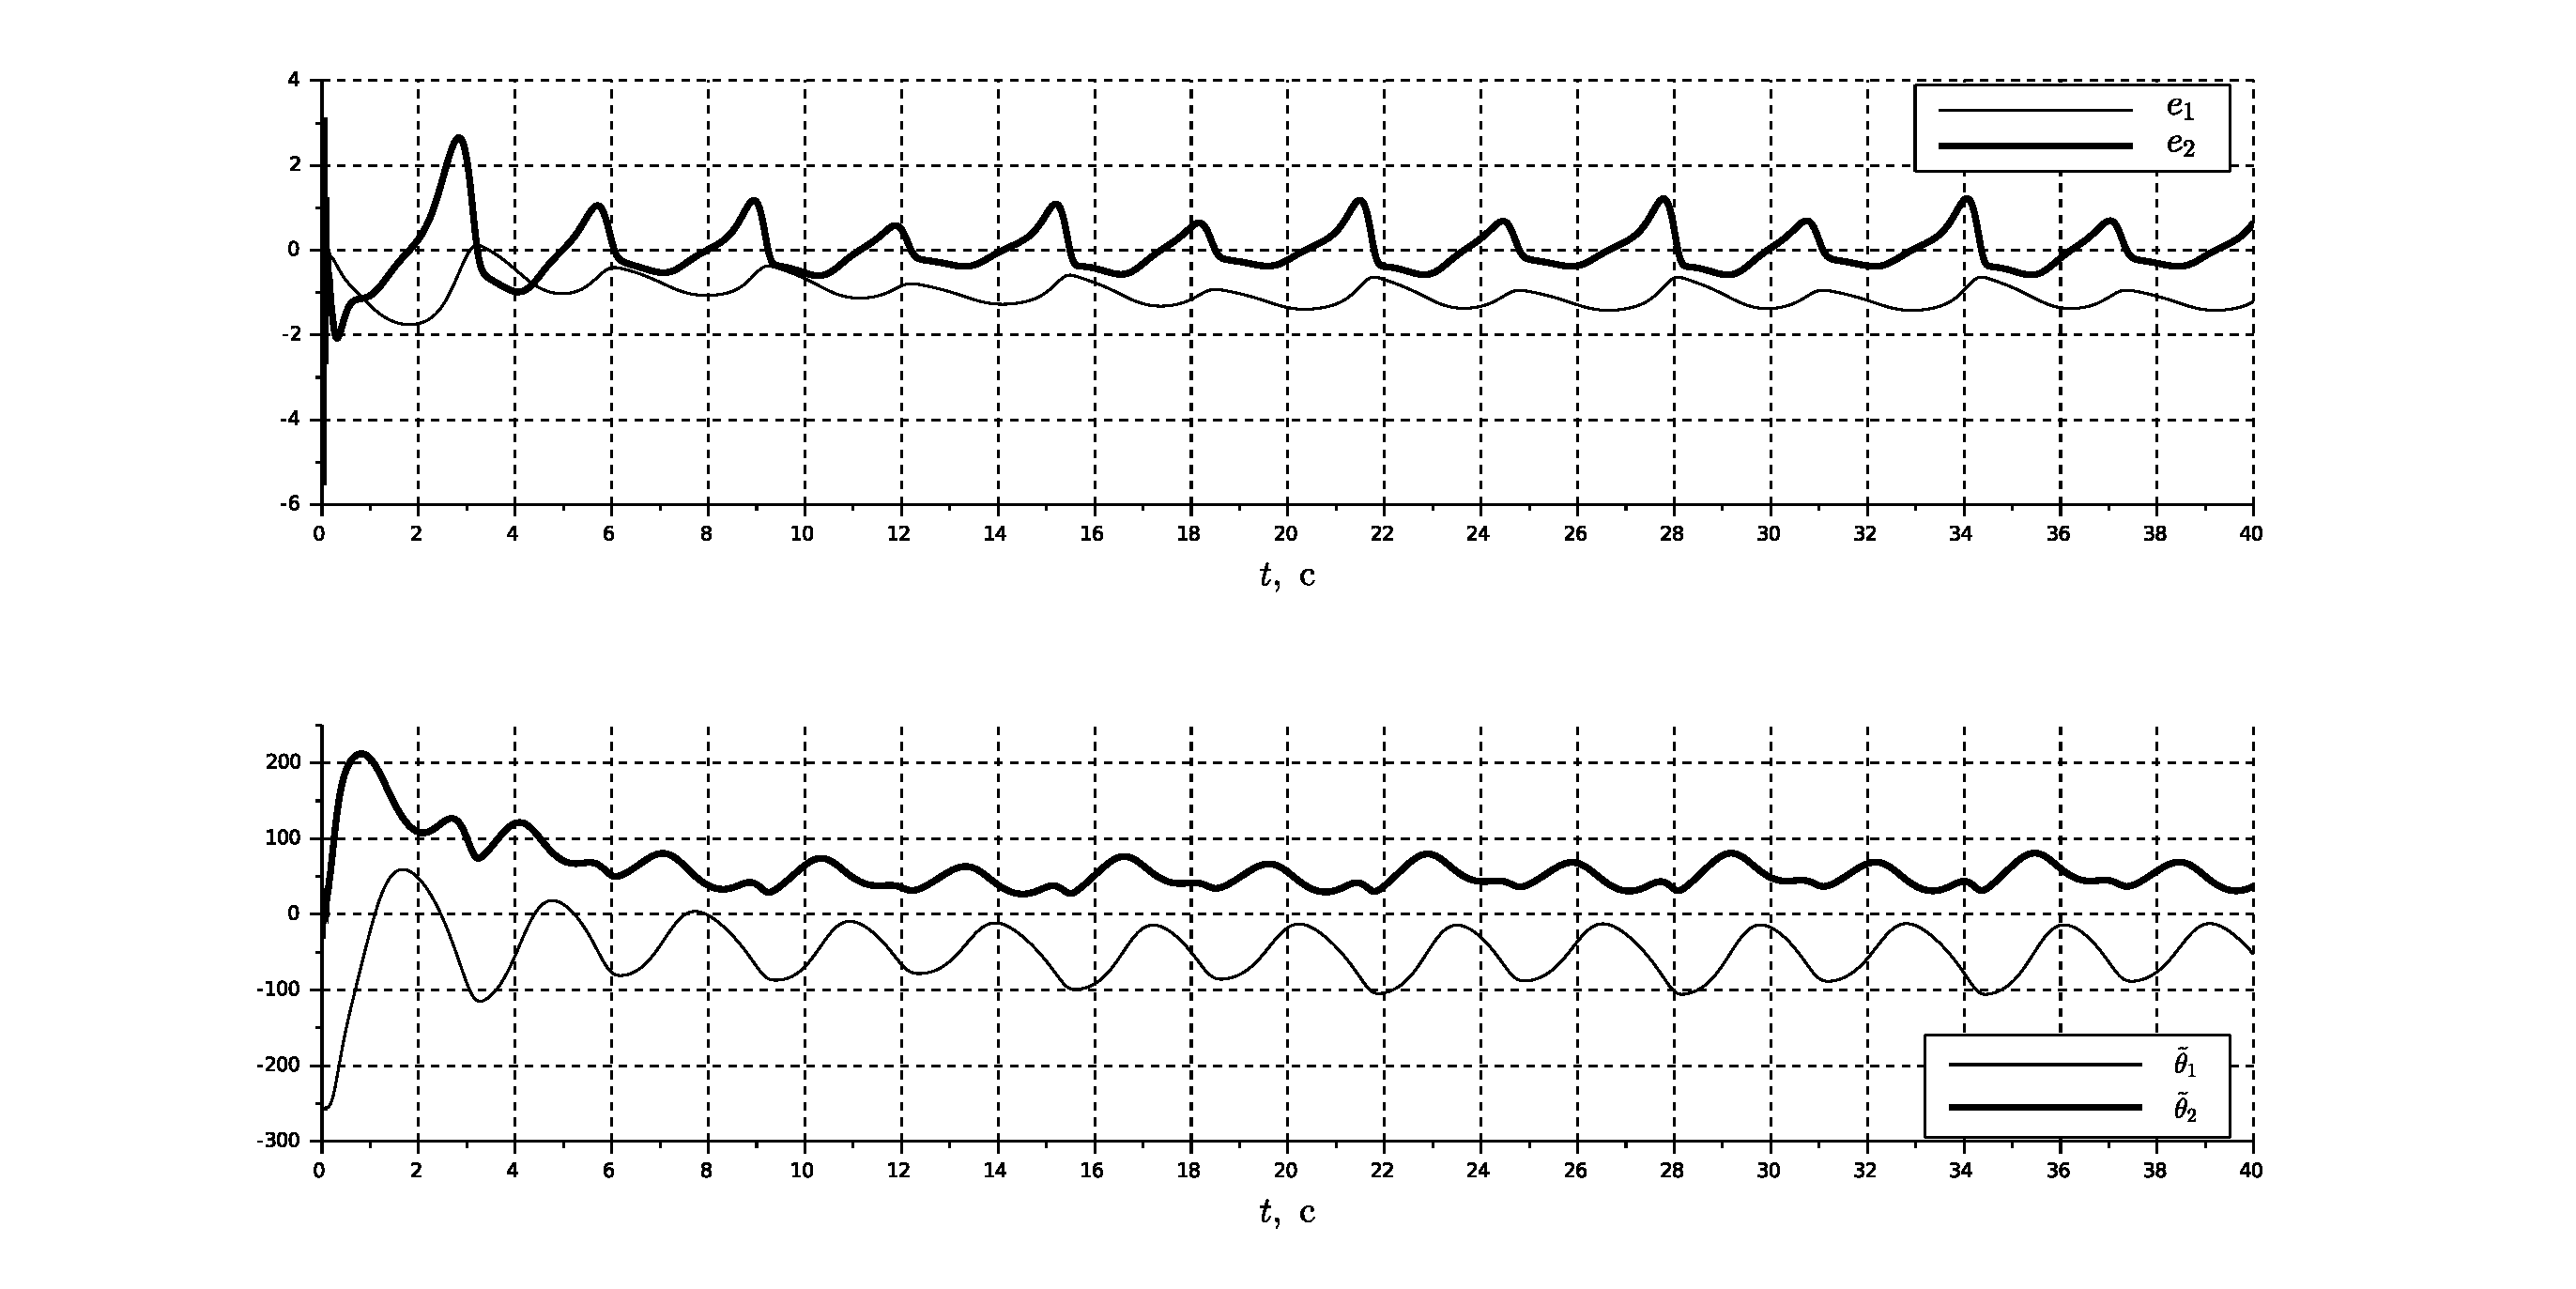
\includegraphics[width=1\textwidth]{arobust_1500_2.pdf}
	\caption{Графики ошибок вектора состояния и параметров невозмущенной системы при $\sigma = 0.2, \gamma = 1500$}
	\label{img_ar1500_2}
\end{figure}

\begin{figure}[h!]
	\centering
	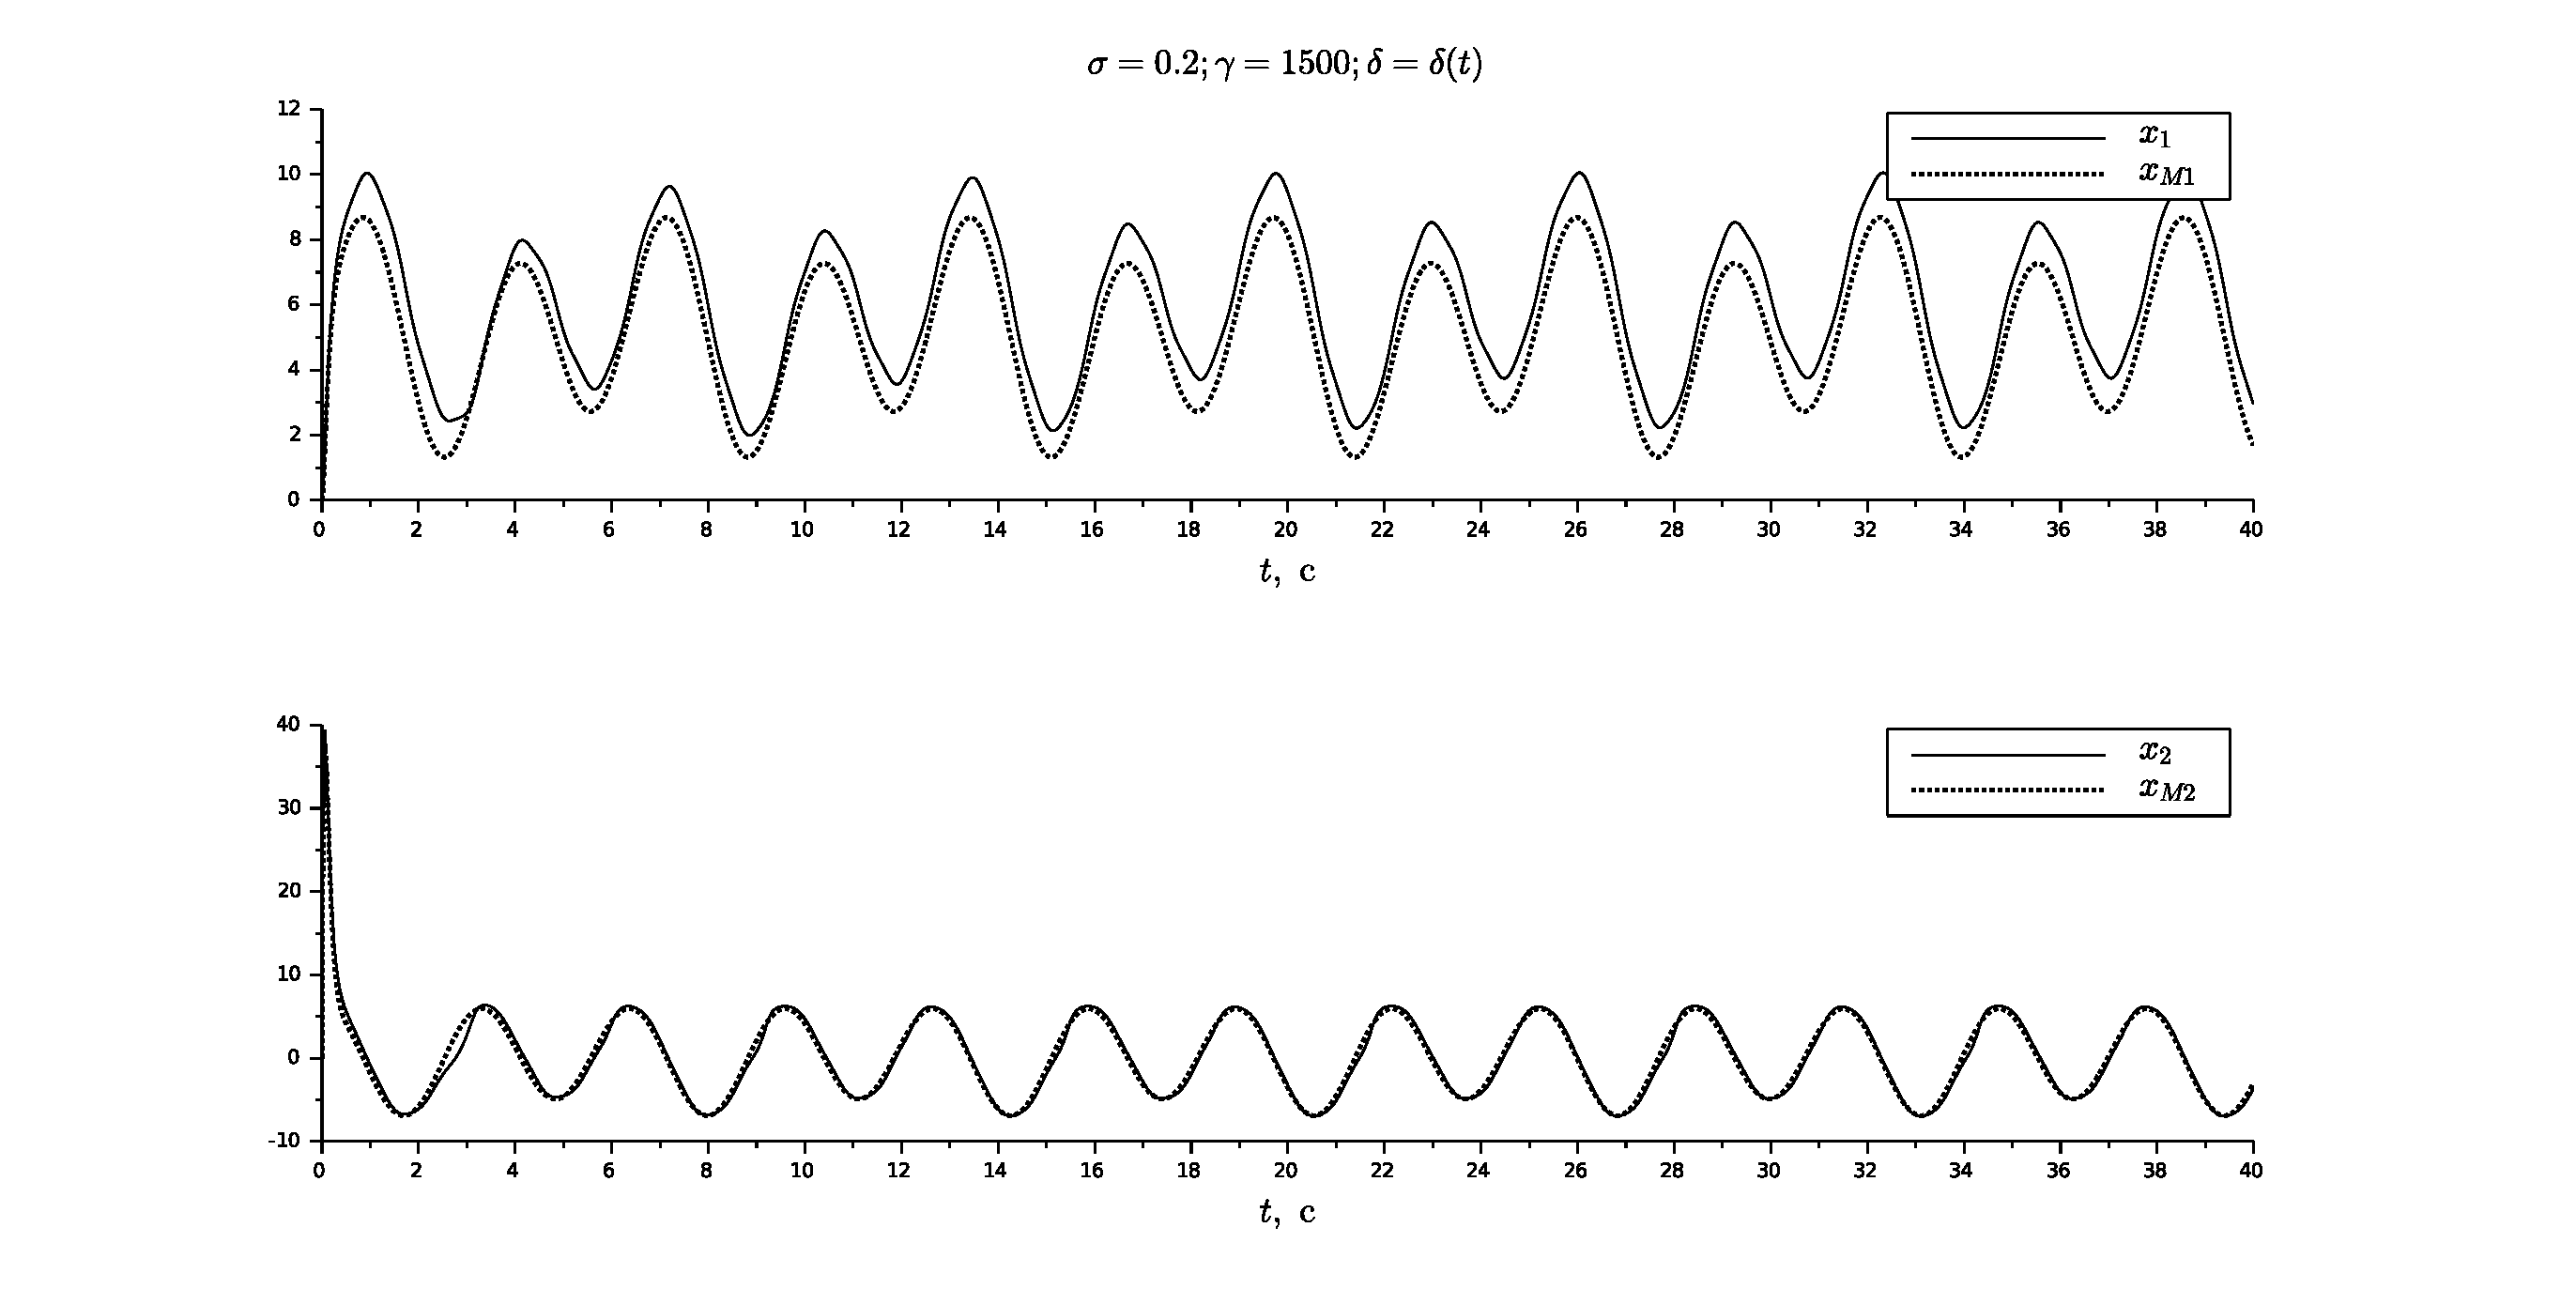
\includegraphics[width=1\textwidth]{arobust_1500_d_1.pdf}
	\caption{Графики переходных процессов возмущенной системы при $\sigma = 0.2, \gamma = 1500$}
	\label{img_ar1500d}
\end{figure}

\begin{figure}[h!]
	\centering
	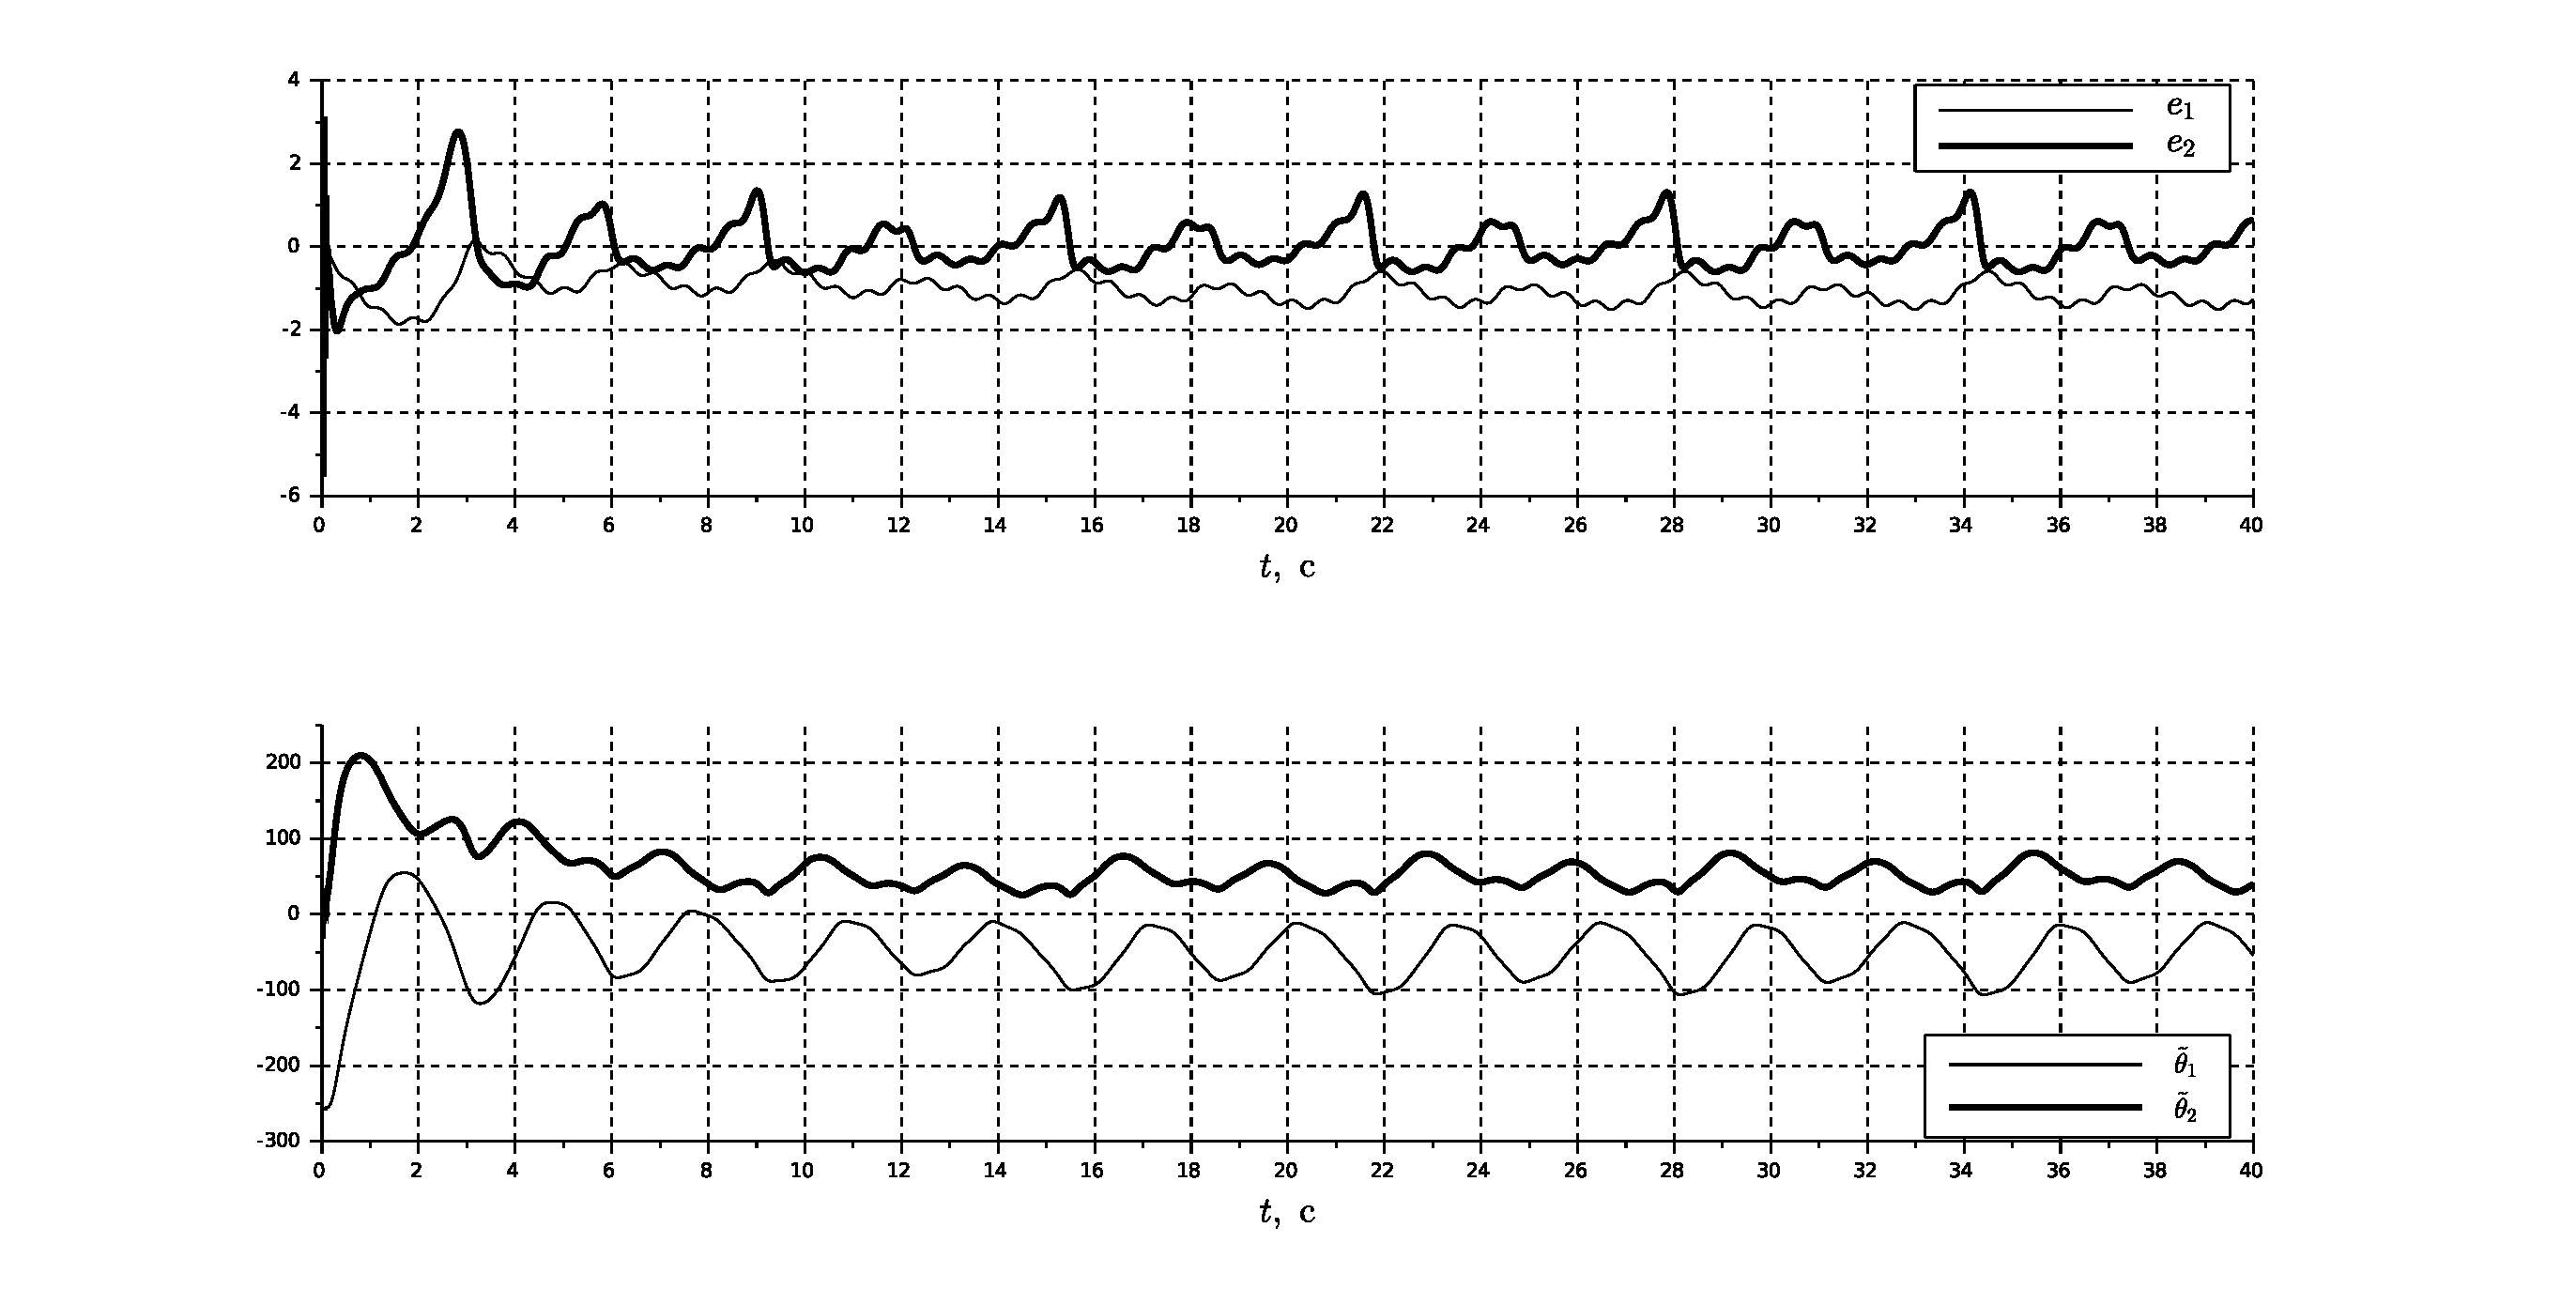
\includegraphics[width=1\textwidth]{arobust_1500_d_2.pdf}
	\caption{Графики ошибок вектора состояния и параметров возмущенной системы при $\sigma = 0.2, \gamma = 1500$}
	\label{img_ar1500_d2}
\end{figure}


\begin{figure}[h!]
	\centering
	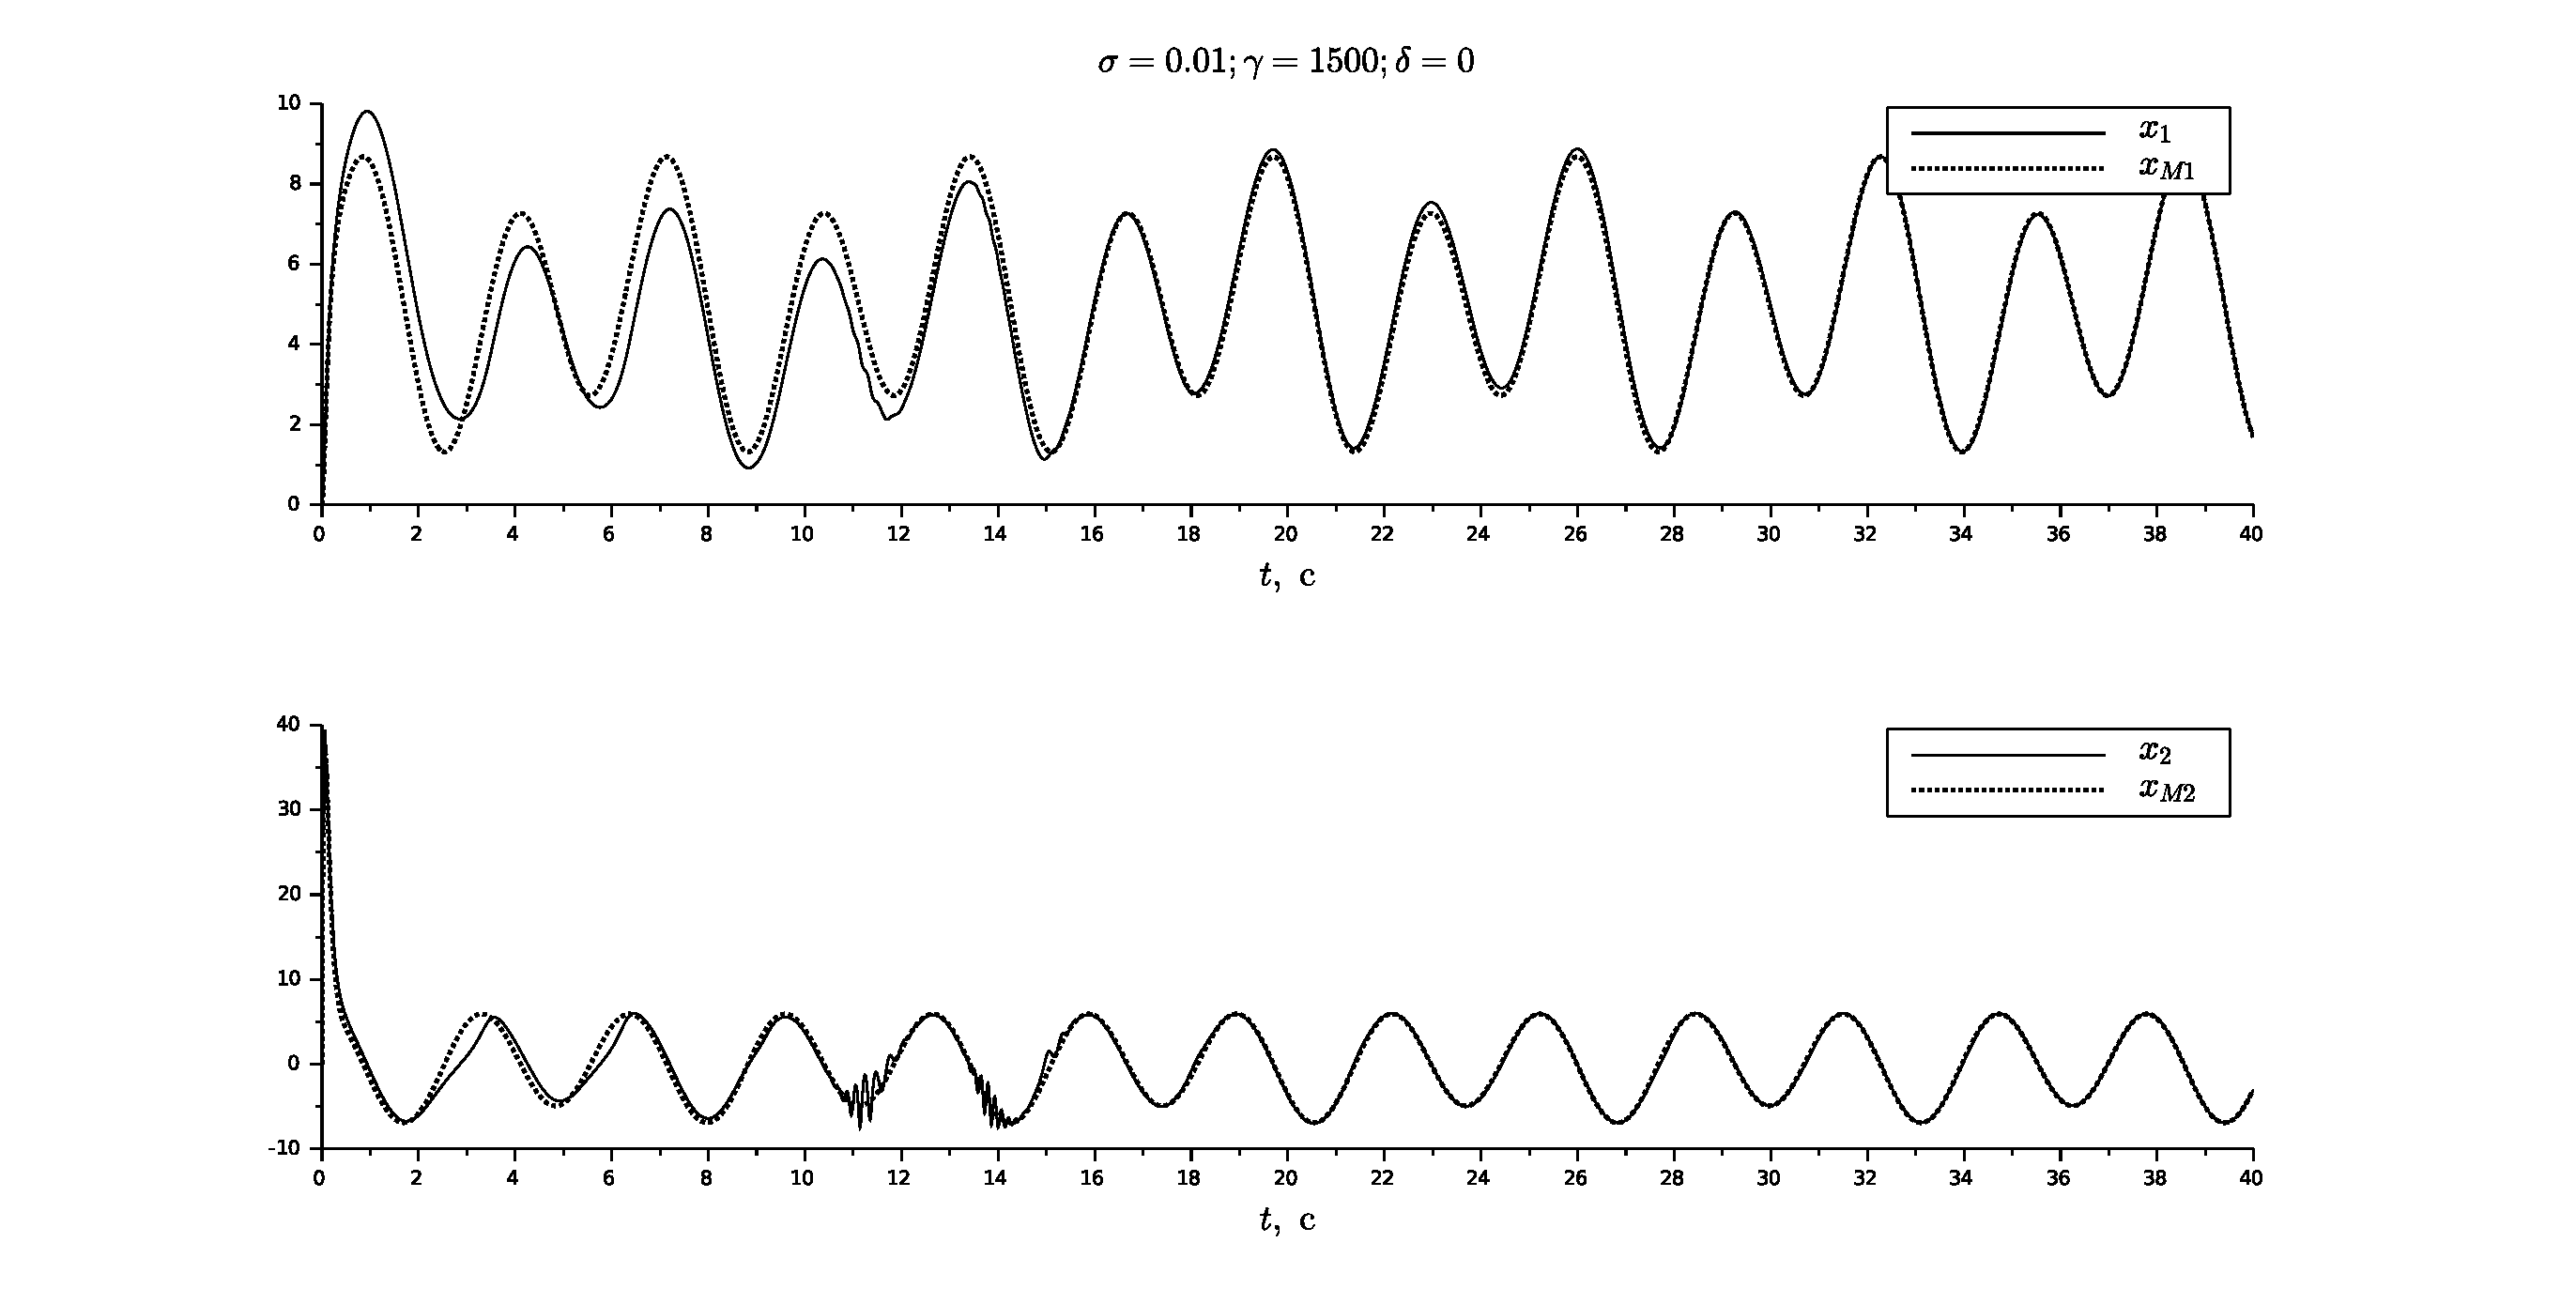
\includegraphics[width=1\textwidth]{s01arobust_1500_1.pdf}
	\caption{Графики переходных процессов невозмущенной системы при $\sigma = 0.01, \gamma = 1500$}
	\label{img_s01ar1500}
\end{figure}

\begin{figure}[h!]
	\centering
	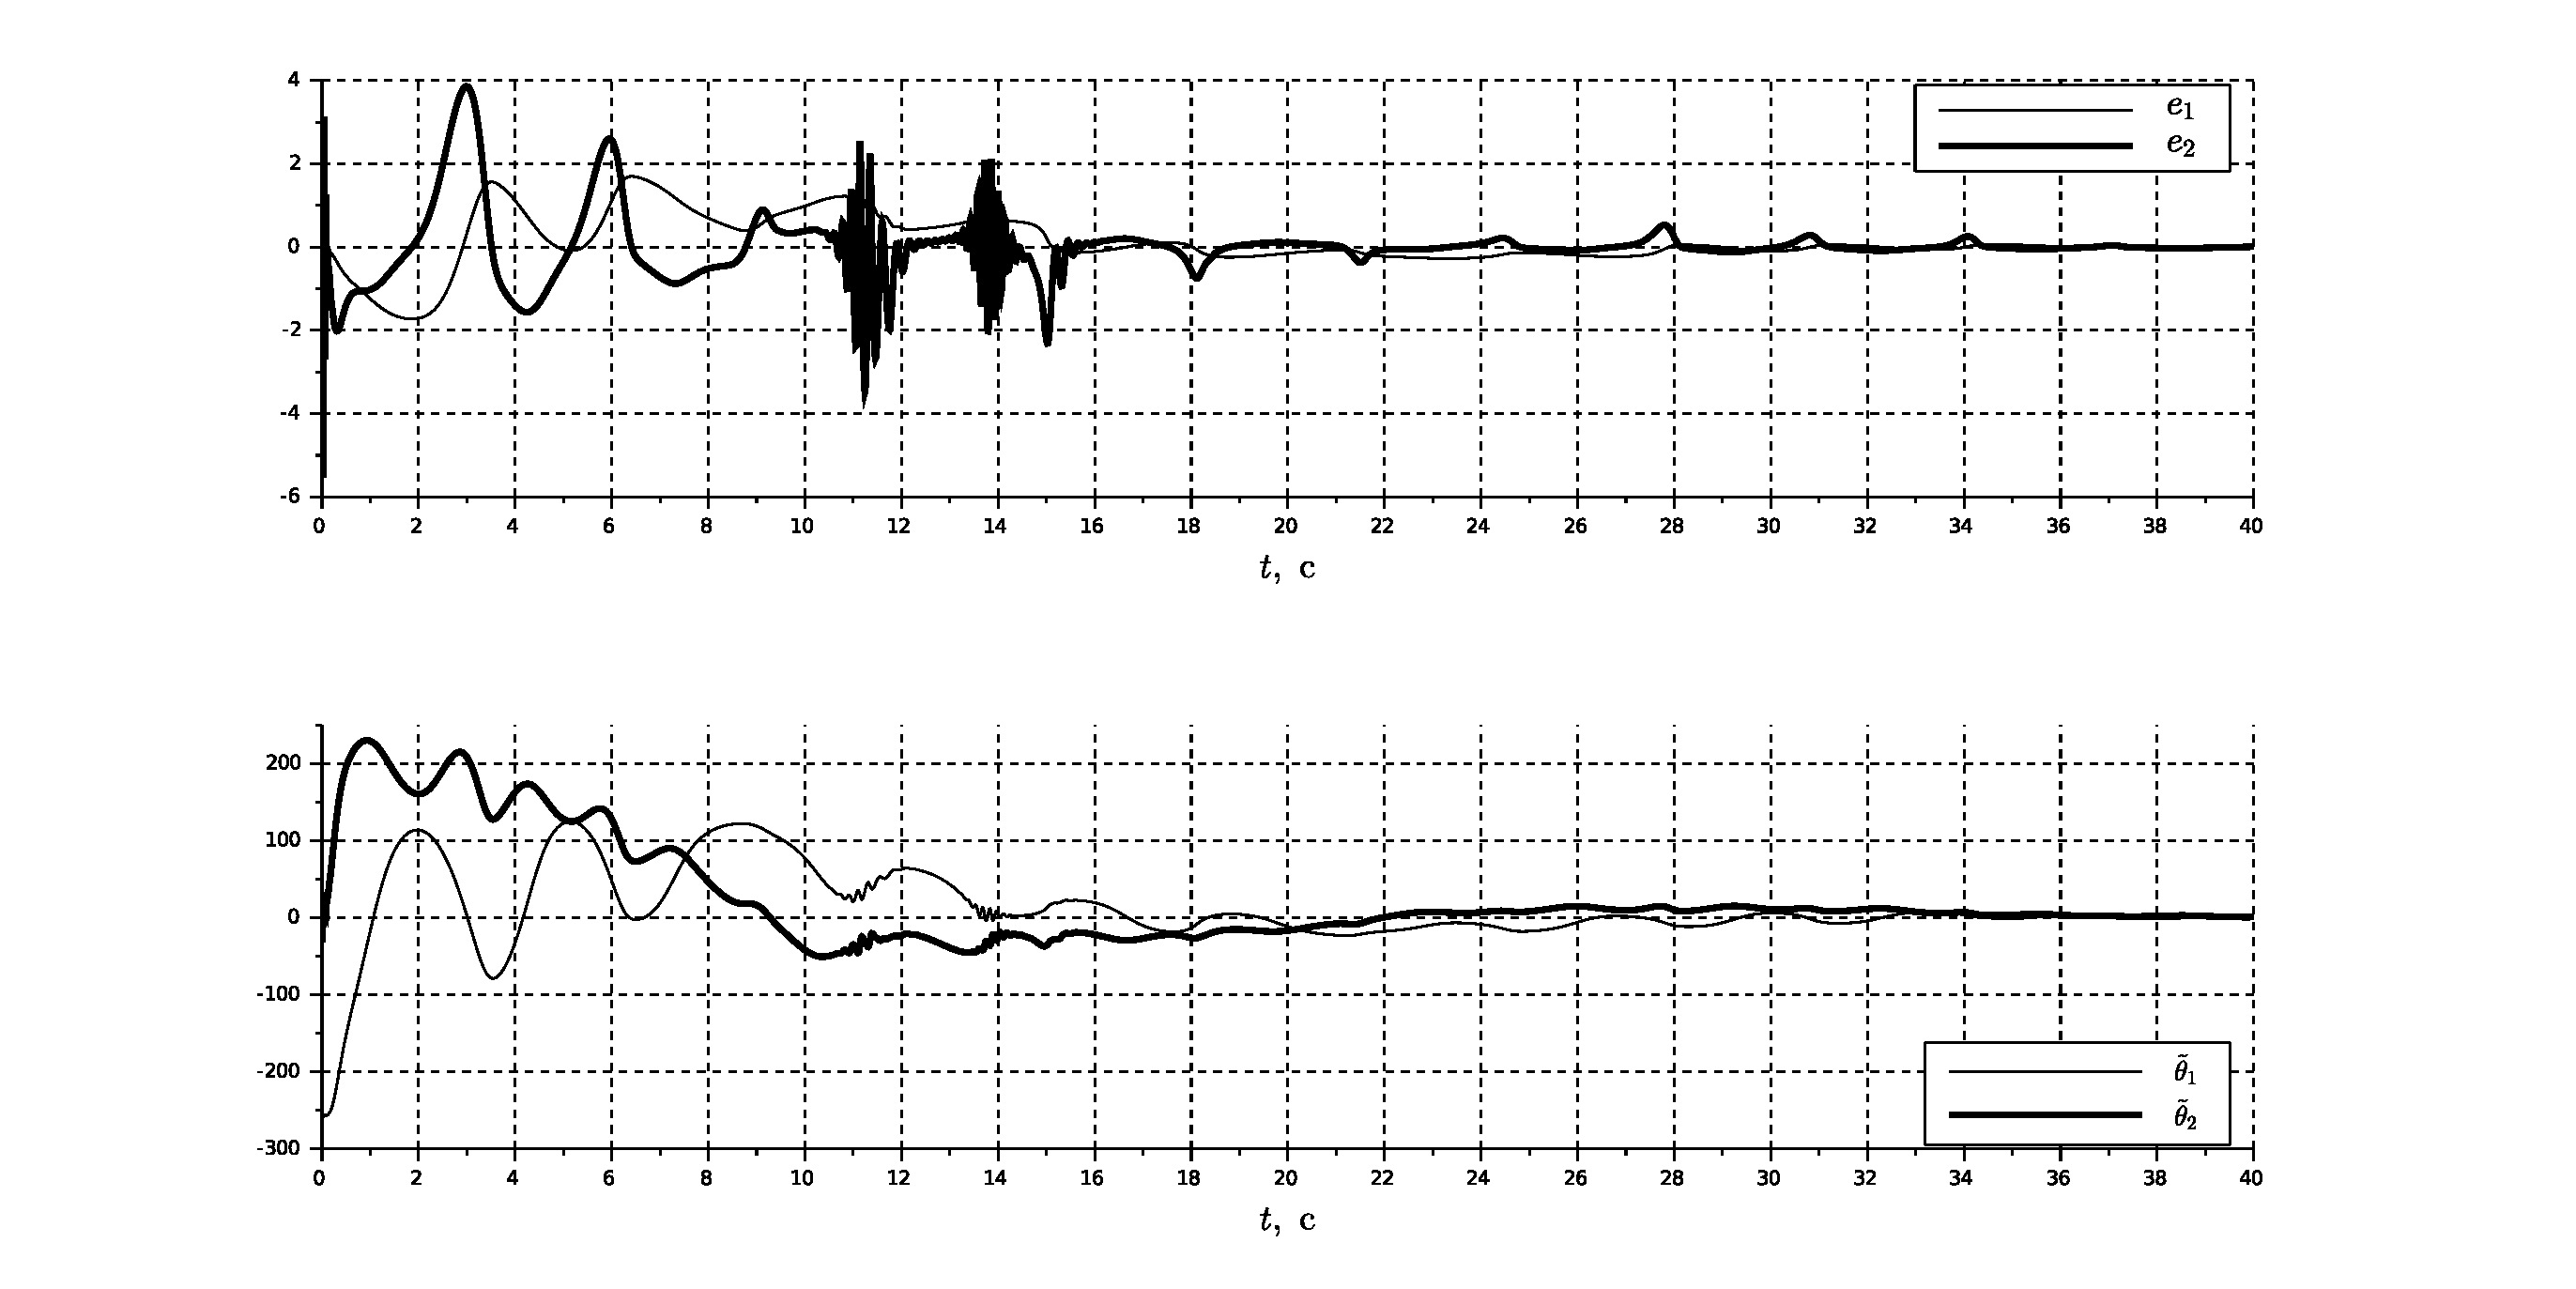
\includegraphics[width=1\textwidth]{s01arobust_1500_2.pdf}
	\caption{Графики ошибок вектора состояния и параметров невозмущенной системы при $\sigma = 0.01, \gamma = 1500$}
	\label{img_s01ar1500_2}
\end{figure}

\begin{figure}[h!]
	\centering
	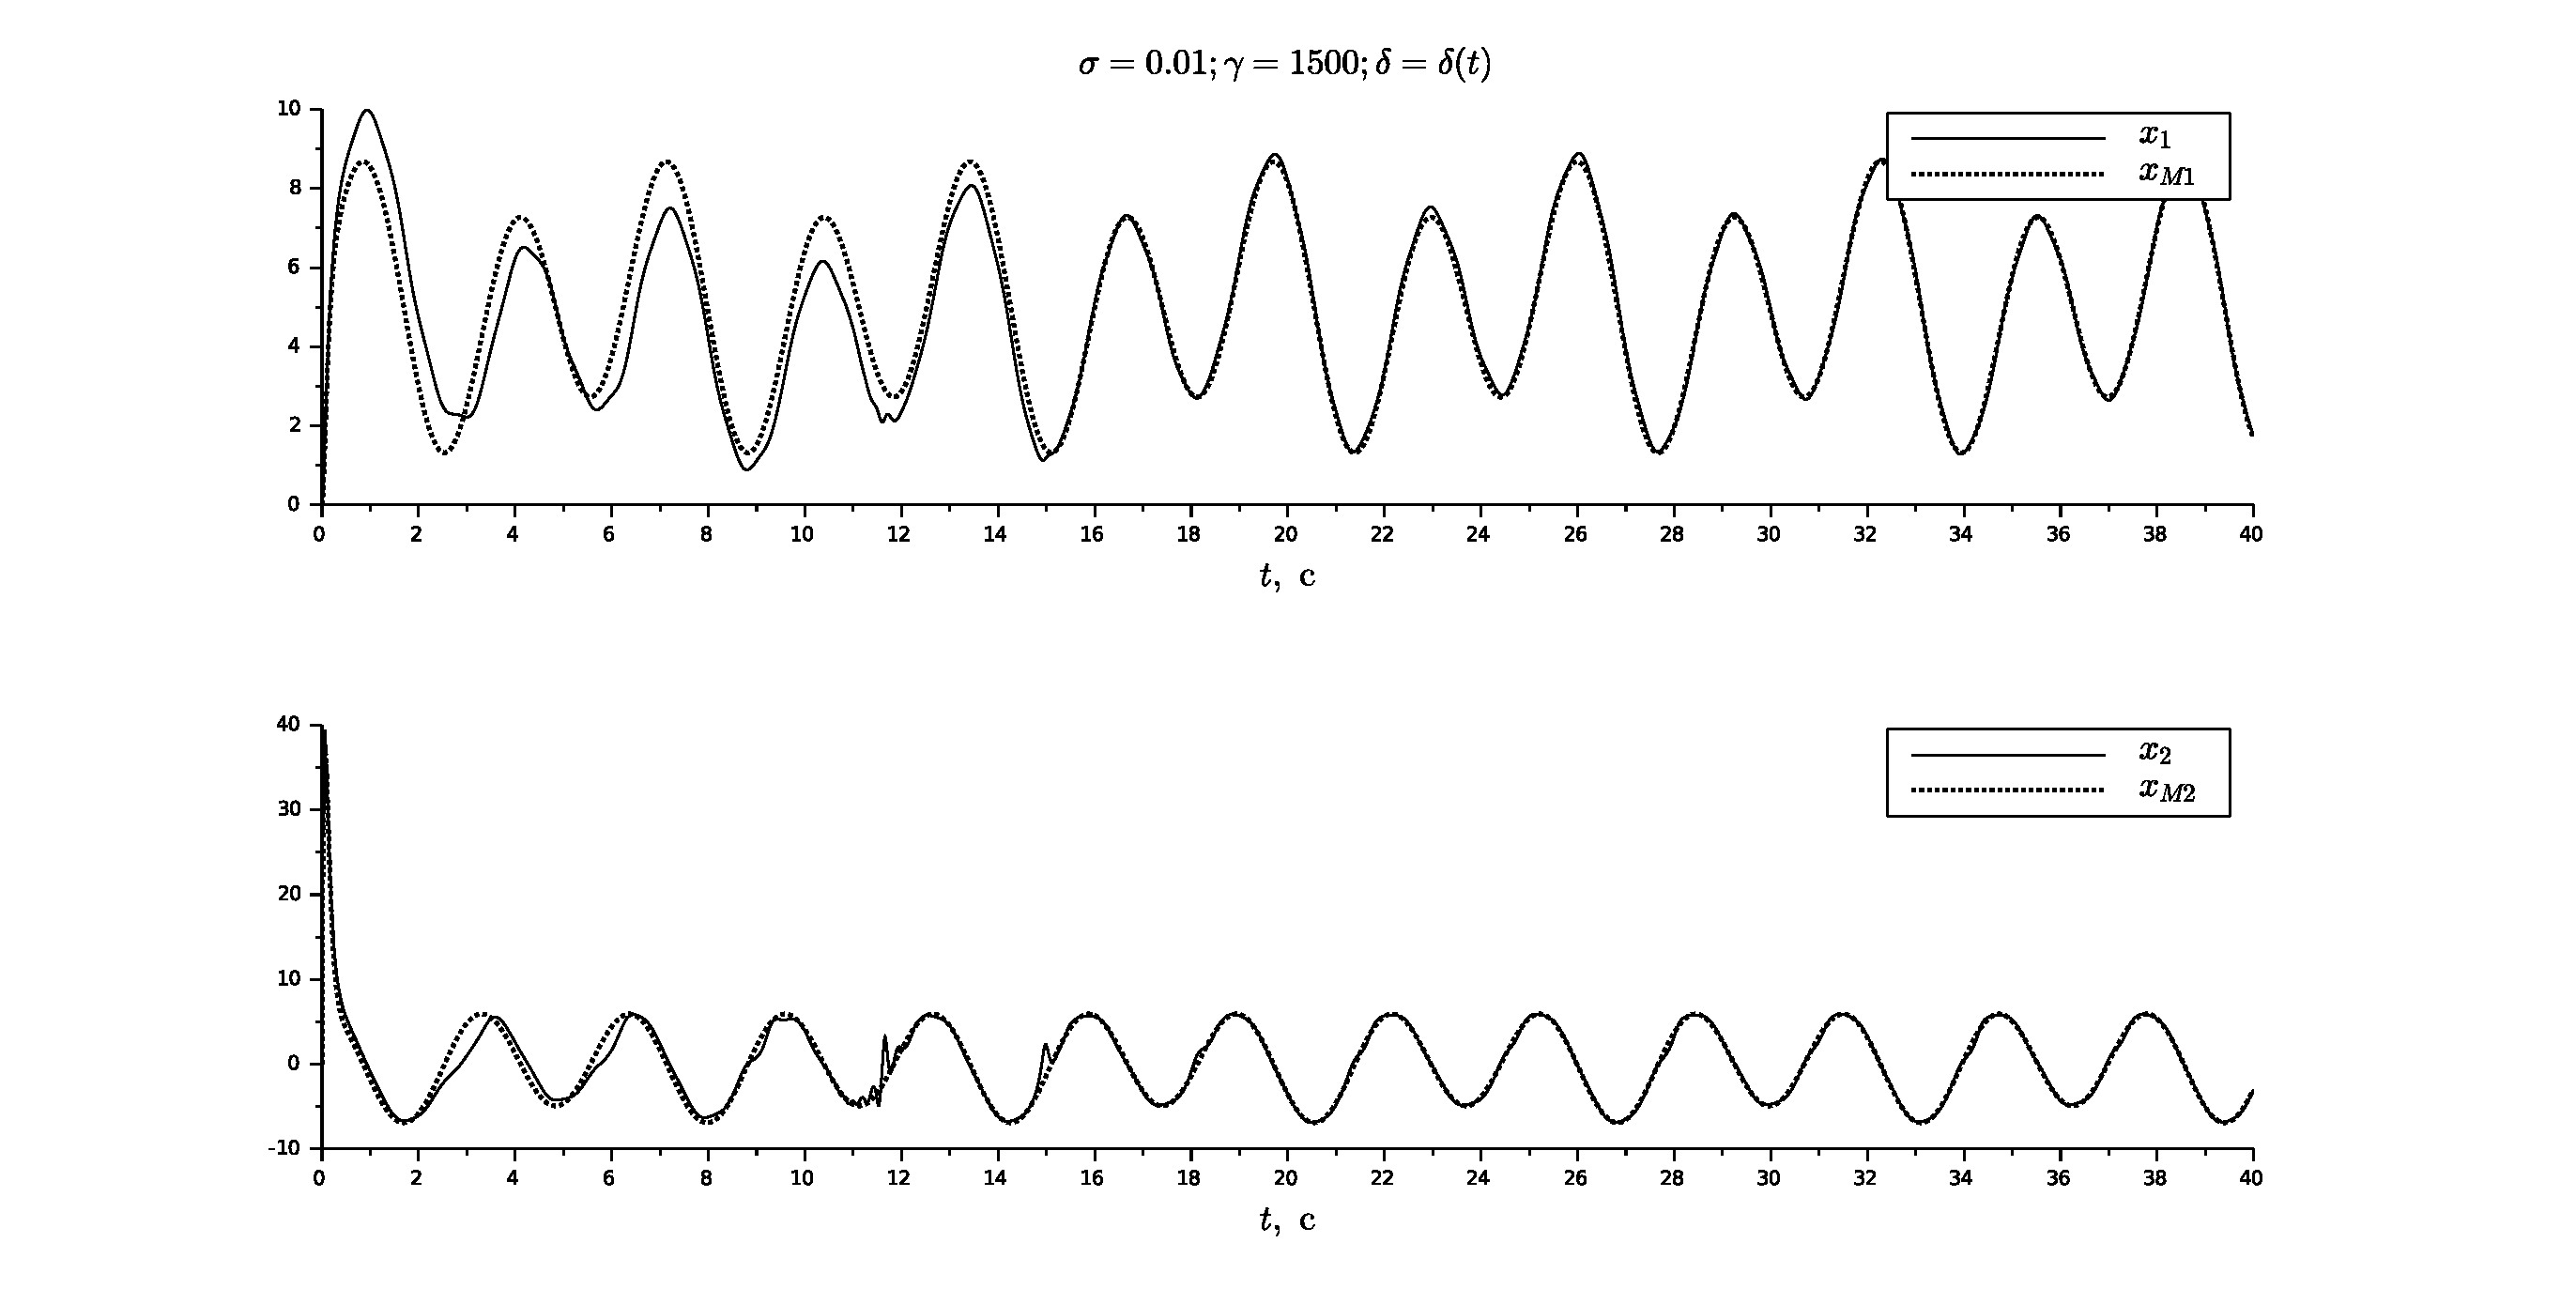
\includegraphics[width=1\textwidth]{s01arobust_1500_d_1.pdf}
	\caption{Графики переходных процессов возмущенной системы при $\sigma = 0.01, \gamma = 1500$}
	\label{img_s01ar1500d}
\end{figure}

\begin{figure}[h!]
	\centering
	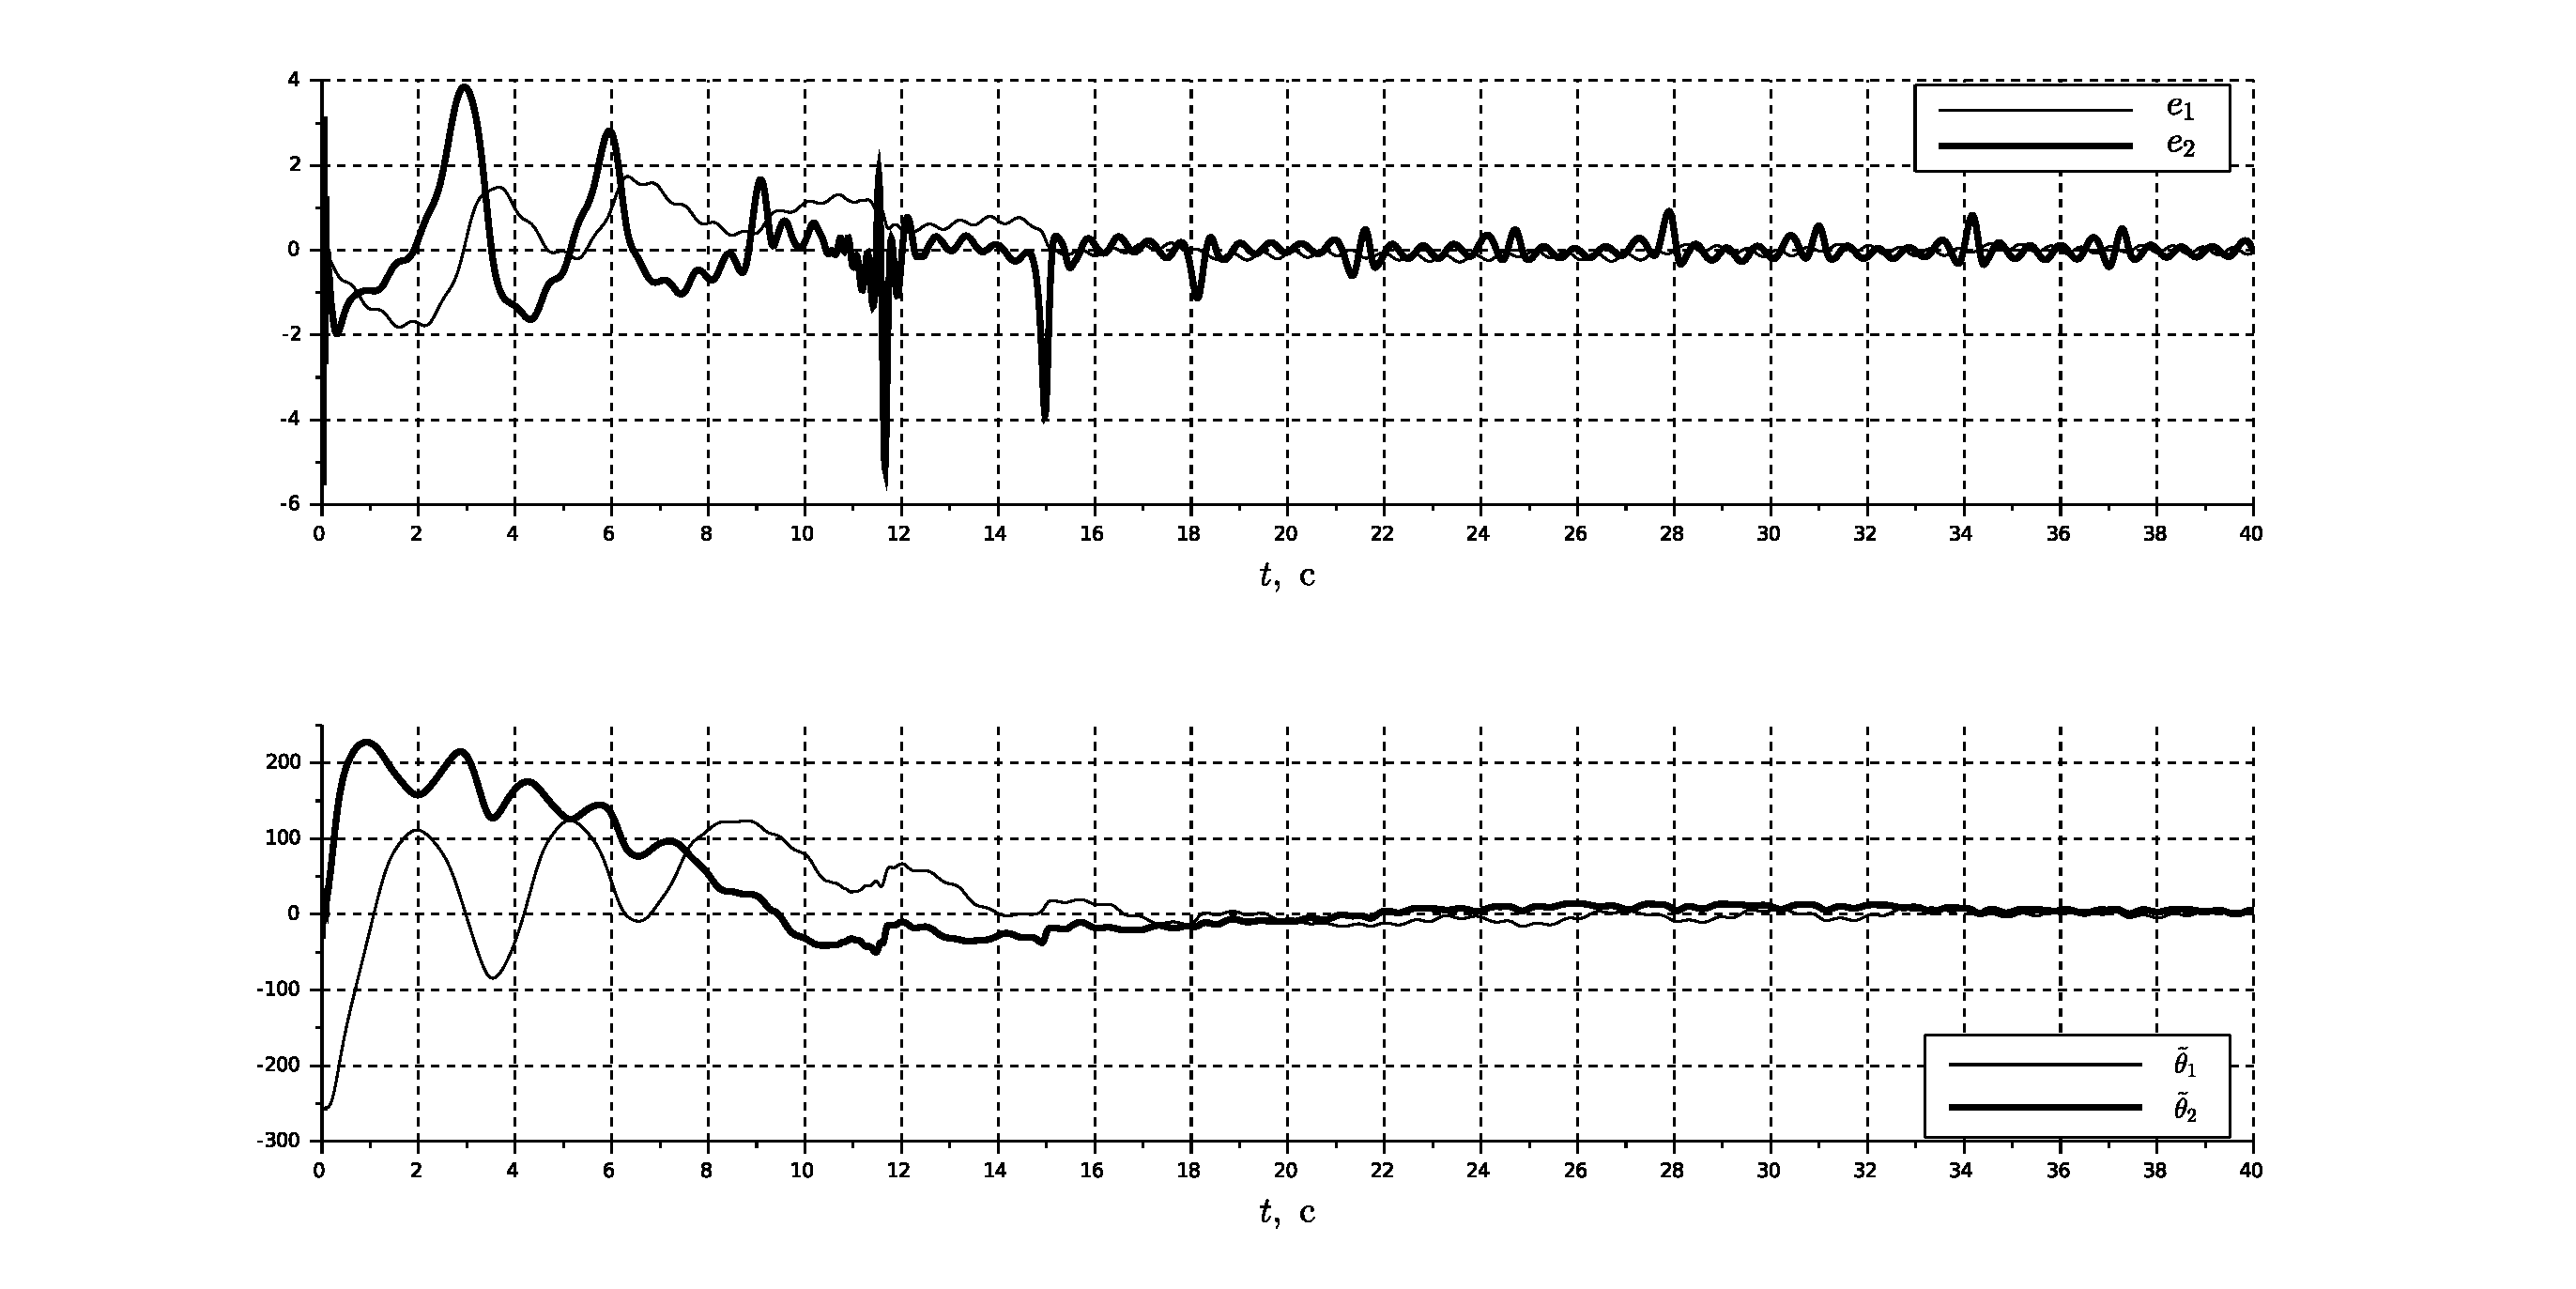
\includegraphics[width=1\textwidth]{s01arobust_1500_d_2.pdf}
	\caption{Графики ошибок вектора состояния и параметров возмущенной системы при $\sigma = 0.01, \gamma = 1500$}
	\label{img_s01ar1500_d2}
\end{figure}


\newpage
\mbox{}
\newpage
\clearpage
\section{Выводы по работе}
В~результате проделанной работы было экспериментально установлено, что 
\begin{enumerate}
	\item оба АА обеспечивают устойчивость замкнутой системы и робастность по отношению к внешнему возмущению;
	\item экспоненциальную сходимость нормы вектора ошибки $e$ к ограниченно окрестности нулевого положения равновесия. Радиус этой окрестности можно уменьшить путем увеличения коэффициента адаптации $\gamma$, и, в случае АА~\ref{AA2}, уменьшением значения $\sigma$;
	\item в случае АА~\ref{AA1}, как и в Лабораторной работе №2, при отсутствии внешнего возмущающего воздействия установившаяся ошибка $e(t)$ отлична от нуля.
\end{enumerate}
